\documentclass[11pt,fleqn]{article}
\usepackage[margin=1in,top=1in,bottom=1in]{geometry}
\usepackage{mathtools}
\usepackage{longtable}
\usepackage{enumitem}
\usepackage{hyperref}
\usepackage[dvips]{graphics}
\usepackage[table]{xcolor}
\usepackage{amssymb}
\usepackage{float}
\usepackage{subfig}
\usepackage{booktabs}
%\usepackage{subcaption}

\usepackage[normalem]{ulem}

\usepackage{multicol}
\usepackage{txfonts}
\usepackage{amsfonts}
\usepackage{natbib}
\usepackage{gb4e}
\usepackage[all]{xy}
\usepackage{rotating}
\usepackage{tipa}
\usepackage{multirow}
\usepackage{authblk}
\usepackage{url}
\usepackage{pdflscape}
\usepackage{rotating}
\usepackage{adjustbox}
\usepackage{array}

\def\bad{{\leavevmode\llap{*}}}
\def\marginal{{\leavevmode\llap{?}}}
\def\verymarginal{{\leavevmode\llap{??}}}
\def\swmarginal{{\leavevmode\llap{4}}}
\def\infelic{{\leavevmode\llap{\#}}}

\definecolor{airforceblue}{rgb}{0.36, 0.54, 0.66}

\newcommand{\dashrule}[1][black]{%
  \color{#1}\rule[\dimexpr.5ex-.2pt]{4pt}{.4pt}\xleaders\hbox{\rule{4pt}{0pt}\rule[\dimexpr.5ex-.2pt]{4pt}{.4pt}}\hfill\kern0pt%
}

\setlength{\parindent}{.3in}
\setlength{\parskip}{0ex}

\newcommand{\yi}{\'{\symbol{16}}}
\newcommand{\nasi}{\~{\symbol{16}}}
\newcommand{\hina}{h\nasi na}
\newcommand{\ina}{\nasi na}

\newcommand{\foc}{$_{\mbox{\small F}}$}

\hyphenation{par-ti-ci-pa-tion}

\setlength{\bibhang}{0.5in}
\setlength{\bibsep}{0mm}
\bibpunct[:]{(}{)}{,}{a}{}{,}

\newcommand{\6}{\mbox{$[\hspace*{-.6mm}[$}} 
\newcommand{\9}{\mbox{$]\hspace*{-.6mm}]$}}
\newcommand{\sem}[2]{\6#1\9$^{#2}$}
\renewcommand{\ni}{\~{\i}}

\newcommand{\citepos}[1]{\citeauthor{#1}'s \citeyear{#1}}
\newcommand{\citeposs}[1]{\citeauthor{#1}'s}
\newcommand{\citetpos}[1]{\citeauthor{#1}'s (\citeyear{#1})}

\newcolumntype{R}[2]{%
    >{\adjustbox{angle=#1,lap=\width-(#2)}\bgroup}%
    l%
    <{\egroup}%
}
\newcommand*\rot{\multicolumn{1}{R{90}{0em}}}% no optional argument here, please!


\title{What is a `factive' predicate? \\ On the empirical purview of projection analyses\thanks{For helpful comments on the research presented here, we thank David Beaver, Kai von Fintel, Mandy Simons, the anonymous reviewers for {\em Semantics and Linguistic Theory} 2018, as well as the audiences at the MIT Linguistics colloquium and the 2018 Annual Meeting of XPRAG.de. We gratefully acknowledge financial support for this research from {\em National Science Foundation} grant BCS-1452674 (JT) and the Targeted Investment for Excellence Initiative at The Ohio State University (JT).}}

\author[$\circ$]{Judith Tonhauser}
\author[$\bullet$]{Judith Degen}

\affil[$\circ$]{The Ohio State University / University of Stuttgart}
\affil[$\bullet$]{Stanford University}

\renewcommand\Authands{ and }

\newcommand{\jt}[1]{\textbf{\color{blue}JT: #1}}

\begin{document}

%\tableofcontents
%\newpage

\maketitle


\begin{abstract}

A `factive' predicate is standardly defined as one for which the content of the clausal complement is both projective and entailed, such as {\em know} or {\em discover}, whereas it is not both projective and entailed for `non-factive' predicates, like {\em think} or {\em inform}. This paper argues, based on the findings of experiments designed to explore projectivity and entailment with 20 `factive' and `non-factive' English clause-embedding predicates, that `factive' predicates are heterogeneous and that the assumed categorical distinction between `factive' and `non-factive' predicates is not supported empirically. As a consequence, it is not empirically justified for analyses of the projectivity of the content of the complement of clause-embedding predicates to be limited to `factive' predicates (see, e.g., \citealt{heim83,vds92,abrusan2011,abrusan2016,romoli2015} and \citealt{best-question}). We show that no currently available projection analysis accounts for our findings and discuss the implications of our findings for empirically adequate analyses of projection.

\end{abstract}
			
\section{Introduction}\label{s1}

Projective content is utterance content that the speaker may be taken to be committed to even when the expression that contributes the content occurs in an entailment-canceling environment (e.g., \citealt{brst-salt10,brst-lang11,tbd-variability}). To illustrate, consider the examples in (\ref{know}) and (\ref{know2}). Since (\ref{know}) is typically taken to entail the content of the complement of {\em know}, that Julian dances salsa, the speaker of (\ref{know}) is taken to be committed to this content. The so-called family-of-sentences variants of (\ref{know}) given in (\ref{know2}a-d) do not entail this content because {\em know} and its clausal complement occur in an entailment-canceling environment: under negation in (\ref{know2}a), in a polar question in (\ref{know2}b), under the epistemic possibility modal {\em perhaps} in (\ref{know2}c) and in the antecedent of a conditional in (\ref{know2}d). Since speakers who utter the sentences in (\ref{know2}a-d) may nevertheless be taken to be committed to the truth of the content of the complement, this content, by virtue of being able to `project' over the entailment-canceling operators, is projective content. 

\begin{exe}

\ex\label{know} Sandra knows that Julian dances salsa.

\ex\label{know2} 

\begin{xlist} 
\ex Sandra doesn't know that Julian dances salsa. 
\ex Does Sandra know that Julian dances salsa?
\ex Perhaps Sandra knows that Julian dances salsa.
\ex If Sandra knows that Julian dances salsa, she'll ask him to dance. 
\end{xlist}

\end{exe}

In contrast, speakers who utter one of the variants of (\ref{know}) and (\ref{know2}) with {\em think} in (\ref{think}) and (\ref{think2}), respectively, are not typically taken to be committed to the truth of the content of the complement, that Julian dances salsa. In other words, the content of the complement of {\em think} is not entailed by (\ref{think}) and (generally assumed to be) not projective in (\ref{think2}).

\begin{exe}

\ex\label{think} Sandra thinks that Julian dances salsa.
\ex\label{think2} 

\begin{xlist} 
\ex Sandra doesn't think that Julian dances salsa. 
\ex Does Sandra think that Julian dances salsa?
\ex Perhaps Sandra thinks that Julian dances salsa.
\ex If Sandra thinks that Julian dances salsa, she'll ask him to dance. 
\end{xlist}

\end{exe}

These differences in the interpretation of sentences with {\em know} and {\em think} are illustrative of a widely-adopted distinction that has been made for a long time among clause-embedding predicates (e.g., \citealt{karttunen71b,kiparsky-kiparsky71}): as defined in (\ref{def}), the content of the complement of so-called `factive' predicates, like {\em know} or {\em discover}, is both entailed and projective, and the content of the complement of `non-factive' predicates, like {\em think} or {\em inform},  is not both entailed and projective. 

\begin{exe}
\ex\label{def} Let $S$ be an unembedded matrix sentence in which a clause $C$ is the argument of a clause-embedding predicate $P$. The clause-embedding predicate $P$ is {\bf factive} if and only if the content of $C$ is

\begin{xlist}
\ex entailed by the content of $S$ and
\ex projective in utterances of family-of-sentence variants of $S$.
\end{xlist}
Otherwise, the predicate is {\bf non-factive}.
\end{exe}

Given the definition in (\ref{def}), `factive' predicates are a homogenous class of predicates (the content of the complement is both entailed and projective), but `non-factive' predicates are a heterogeneous class. For a first subset henceforth called `plain non-factives', including {\em think} and {\em pretend}, the content of the complement is neither entailed nor projective, as illustrated in (\ref{think}) and (\ref{think2}) for {\em think}. For a second subset, including {\em be right}, the content of the complement is entailed but not projective; we refer to these predicates as `veridical non-factives'. Thus, the content of (\ref{right}) is generally taken to entail the content of the complement, but speakers who utter one of the family-of-sentences variants in (\ref{right2}) are not taken to be committed to the content of the complement, which means that it is not projective. 

\begin{exe}
\ex\label{right} Sandra is right that that Julian dances salsa.
\ex\label{right2} 

\begin{xlist} 
\ex Sandra isn't right that Julian dances salsa. 
\ex Is Sandra right that Julian dances salsa?
\ex Perhaps Sandra is right that Julian dances salsa.
\ex If Sandra is right that Julian dances salsa, she'll ask him to dance. 
\end{xlist}
\end{exe}
Finally, for a third subset of `non-factive' predicates, including {\em announce, tell, confess, establish, inform, acknowledge, admit} and {\em confirm}, the content of the complement is projective but not entailed; for comments to this effect see, e.g., \citealt{reis1973,melvold1991,schultz2003,swanson2012,anand-hacquard2014,spector-egre2015,karttunen2016,tbd-variability}.  We refer to these `non-factive' predicates as `projective non-factive'. Consider the sentence in (\ref{announce2}a) with {\em announce}. As pointed out by \citet[139]{schlenker10}, if Mary is a responsible 30-year old woman, then speakers who utter (\ref{announce2}a) may very well be taken to be committed to the content of the complement, that Mary is pregnant, i.e., this content is projective. That the content of the complement of {\em announce} is not entailed, and {\em announce} therefore is a `non-factive' predicate, can be seen from the fact that, if Mary is a 7-year old girl, speakers who utter (\ref{announce2}b)  are not taken to be committed to Mary being pregnant. 

\begin{exe}
\ex\label{announce2} 
\begin{xlist}
\ex Has Mary announced to her parents that she is pregnant? 
\ex Mary has announced to her parents that she is pregnant. \hfill (\citealt[139]{schlenker10})
\end{xlist}
\end{exe}
Similarly, \citet{spector-egre2015} suggested that it is possible to take a speaker who utters (\ref{tell}a) with the `non-factive' predicate {\em tell}  to be committed to the content of the complement, that Fred is the culprit. That this content is not entailed, and {\em tell} therefore is a `non-factive' predicate, is shown by the fact that the content does not follow from the unembedded variant in (\ref{tell}a) if Sue is known to be an unreliable gossip.

\begin{exe}
\ex\label{tell}
\begin{xlist}
\ex Sue didn't tell Jack that Fred is the culprit. 
\ex Sue told Jack that Fred is the culprit. \hfill (\citealt[1739]{spector-egre2015})
\end{xlist}
\end{exe}

Currently available projection analyses do not make predictions about the projectivity of the content of the complement `projective non-factive' predicates because these analyses are all limited in their empirical scope to `factive' predicates. On \citetpos{heim83} analysis, for instance, the content of the complement of `factive' predicates is lexically specified to be a presupposition, which means that the content is required to be part of the common ground of the interlocutors prior to interpretation. The content of the complement of `projective non-factive' predicates does not carry this lexical specification and, as a consequence, the analysis makes no predictions about the projectivity of the content of the complement of `projective non-factive' (or other `non-factive') predicates. On the analyses developed in \citealt{abrusan2011,abrusan2016}, \citealt{romoli2015} and \citealt{best-question}, the projectivity of the content of the complement of `factive' predicates is derived from its status as entailed content: on Abrus\'an's (2011, 2016) analysis, for instance, the entailed content of the complement is, by default, backgrounded and therefore projective, and on \citetpos{best-question} analysis, questions addressed by utterances with `factive' predicates can entail the content of the complement, which is thereby projective. Because the content of the complement of  `projective non-factive' predicates is not entailed, these analyses do not make predictions about the projectivity of this content. 

Other authors make predictions about the projectivity of the content of the complement of `projective non-factive' predicates by assimilating them to `factive' predicates. \citet[139]{schlenker10}, for instance, proposed that {\em announce} is a ``part-time presupposition trigger'', namely in contexts in which the content of its complement is entailed, thereby allowing the projectivity of the content of its complement to fall in the empirical purview of projection analyses designed for `factive' predicates.\footnote{\citepos{schlenker10} notion of entailment seems to differ from the standard one that is used in this paper in that \citepos{schlenker10} notion is context-sensitive: for instance, he assumes that ``in some contexts, [{\em announce}, JT\&JD] does not entail the truth of its complement; in other contexts, it entails and presupposes the truth of its complement" (p.139).}  Similarly, \citet[1736]{spector-egre2015} proposed that predicates like {\em tell, predict} and {\em announce}  are ambiguous between a lexical entry on which the content of the complement is entailed and another on which it is not; as a consequence, such `projective non-factive' predicates have ``factive uses'' on which the content of the complement is predicted to be projective. Thus, like the analyses reviewed above, \citetpos{schlenker10} and \citetpos{spector-egre2015} projection analyses are essentially limited to `factive' predicates.

Limiting the scope of projection analyses to `factive' predicates is empirically justified if `factive' predicates are an empirically well-grounded class of predicates, for instance, if, as defined in (\ref{def}), the content of their complement is both projective and entailed. In this case, alternative analyses may be called on to predict the projectivity of the content of the complement of `projective non-factive' predicates, which is projective but not entailed. However, based on the findings of experiments designed to explore projectivity and entailment with 20 `factive' and `non-factive' English clause-embedding predicates, we argue in this paper that `factive' predicates are heterogeneous and that the assumed categorical distinction between `factive' and `non-factive' predicates as defined in (\ref{def}) is not supported empirically. As a consequence, we argue, it is not empirically justified for projection analyses to be limited to `factive' predicates.

Reason to doubt that `factive' predicates are a homogenous and empirically well-grounded class of predicates comes  from observations about both projectivity and entailment. Regarding projectivity, it has long been recognized that there is variability in the projectivity of the content of the complement of `factive' predicates. \citet{karttunen71b}, for instance, already suggested that the content of the complement of {\em regret} in (\ref{semi-factive}a) is more projective than that of {\em discover} in (\ref{semi-factive}b): 


\begin{exe}
\ex\label{semi-factive}
\begin{xlist}
\ex John didn't regret that he had not told the truth.
\ex John didn't discover that he had not told the truth.  
\hfill (\citealt[63]{karttunen71b})

\end{xlist}
\end{exe}
More recently, \citet*{tbd-variability} showed that there is even more projection variability than previously assumed, including among presumed `factive' predicates. In particular, they found (Exp.~1b) that the content of the complement of {\em be annoyed, be amused, notice, be aware, realize, see, find out} and {\em learn} was more projective than that of {\em reveal}, which in turn was more projective than that of {\em discover}. In addition to by-predicate variability, they also observed by-participant variability, with only relatively few participants taking the content of the complement of `factive' predicates to be highly projective. Given the observed variability in the projectivity of utterance content, including the content of the complement of `factive' predicates, \citet{tbd-variability} argued that projectivity is not a binary, categorical property of utterance content, but rather a gradient one; see also \citealt{demarneffe-etal2018} for evidence based on naturally occurring examples.  

With respect to the definition of `factive' predicates in (\ref{def}), a consequence of projectivity being a gradient property of utterance content is that it is unclear how projective the content of a complement of a predicate needs to be in order for the predicate to be considered `factive'. 
Furthermore, given that the content of the complement of some `non-factive' predicates is also projective, it is an open question how projective the content of the complement of presumed `factive' predicates is compared to that of presumed `non-factive' predicates. Although \citepos{tbd-variability} experiments were largely limited to `factive' predicates, their Exp.~1b did find that the content of the complement of the `projective non-factive' predicates {\em establish} and {\em confess} was significantly less projective than that of `factive' predicates, albeit still projective when compared to main clause content. Therefore, the first empirical goal of this paper is to systematically explore the projectivity of the content of the complement of a range of English `factive' and `non-factive' predicates. This exploration serves to address the research questions in (\ref{prq}), with the question in (\ref{prq}a) allowing for a comparison with the findings of \citealt{tbd-variability}.

\begin{exe}
\ex\label{prq} Research questions about projectivity
\begin{xlist}
\ex How projective is the content of the complement of `factive' predicates?
\ex How projective is the content of the complement of different kinds of `non-factive' predicates?
\ex Does projectivity distinguish `factive' from `non-factive' predicates?
\end{xlist}
\end{exe}

Reason to doubt that `factive' predicates are a homogenous and empirically well-grounded class of predicates also comes from observations about entailment. Entailment is a binary, categorical relationship between two contents: given sentences $\phi$ and $\psi$, the content of $\phi$ entails the content of $\psi$ if and only if any world in which the content of $\phi$ is true is also a world in which the content of $\psi$ is true. Given this standard definition of the entailment relationship, if there is just one world in which $\phi$ is true but $\phi$ is false, then the content of $\phi$ does not entail the content of $\psi$.

For some clause-embedding predicates, there is disagreement in the literature about whether the content of the complement is entailed. \citet[139]{schlenker10}, for example, assumed that the content of the complement of {\em inform} is entailed, i.e., that Mary being pregnant necessarily follows from (\ref{inform}).  

\begin{exe}
\ex\label{inform} Mary has informed her parents that she's pregnant.

%\ex Mary has announced to her parents that she's pregnant.
\end{exe}
\citet[76]{anand-hacquard2014}, however, pointed out that {\em inform} can be modified by {\em falsely}, as in the naturally occurring example in (\ref{inform2}): crucially, the content of the complement of {\em inform}, that the victims had won more than a million dollars in a lottery, does not follow from (\ref{inform2}). As a consequence, they argue, the content of the complement of {\em inform}  is not entailed and {\em inform} is not a `factive' but a `non-factive' predicate.

\begin{exe}
\ex\label{inform2} From March 2012, Peart's and King's co-conspirators are alleged to have [...] falsely informed [victims] that they had won more than a million dollars in a lottery. \hfill (\citealt[76]{anand-hacquard2014})
\end{exe}
Similarly, both \citet{wyse} and \citet{swanson2012} took the content of the complement of {\em establish} to be entailed, but the naturally occurring example in (\ref{establish}), in which {\em establish} is  modified by {\em falsely}, again shows that this content does not necessarily follow from unembedded matrix sentences with {\em establish}. In other words, (\ref{establish}) suggests that {\em establish} is a `non-factive' predicate.

\begin{exe}
\ex\label{establish} The testimony is uncontradicted that Jew Sing committed at least six perjuries and a subornation of perjury to conceal his wrongful entry into the country, and falsely established that he was an American citizen.\footnote{\url{https://law.justia.com/cases/federal/appellate-courts/F2/202/715/216831/}}
\end{exe}

There is also disagreement about whether the content of the complement of emotive predicates, like {\em be annoyed} or {\em regret}, is entailed. Consider the examples in (\ref{emotive1}), in which two standard diagnostics for entailment are applied to the content of the complement of {\em regret}. First, as noted in \citealt[514]{abrusan2011}, ``from [(\ref{emotive1}a)] one tends to infer that it is raining'', suggesting that the content of the complement is entailed. Second, a speaker who utters the sentence in (\ref{emotive1}b) is judged to contradict themselves (as indicated by the hashmark): it does not seem possible for the speaker to be committed to the proposition that it is not raining and to the proposition that John regrets that it is raining. Examples like these support the position that the content of the  complement of emotive predicates is entailed, as assumed in, e.g., \citealt{gazdar79a,abrusan2011} and \citealt{anand-hacquard2014}.

\begin{exe}

\ex\label{emotive1} \citealt[514]{abrusan2011}

\begin{xlist}

\ex I doubt that John regrets that it's raining.

\ex \infelic It's not raining but John regrets that it's raining. 

\end{xlist}

\end{exe}

There are, however, also examples that show that the content of the complement does not necessarily follow from unembedded matrix sentences with emotive predicates. The content of the complement of {\em regret}, that Oedipus killed the stranger on the road to Thebes, does not follow from (\ref{emotive2}a) and the content of the complement of {\em be enraged}, that Mary is no longer single, does not follow from (\ref{emotive2}b). Some authors, including \citet{klein1975,giannakidou1998,schlenker2003} and \citet{egre2008}, concluded from the existence of examples like those in (\ref{emotive2}) that the content of the complement of emotive predicates is not entailed.

\begin{exe}

\ex\label{emotive2}

\begin{xlist}

\ex Falsely believing that he had inflicted a fatal wound, Oedipus regretted killing the stranger on the road to Thebes \hfill (\citealt{klein1975})

\ex John wrongly believes that Mary got married, and he is enraged that she is no longer single. \\ \hspace*{.2cm} \hfill (adapted from \citealt{egre2008}, based on \citealt{schlenker03})

\end{xlist}

\end{exe}

For other authors, including \citet{gazdar79a} and \citet{abrusan2011}, examples like (\ref{emotive2}) do not constitute evidence that the content of the complement is not entailed. These authors instead suggested that such examples are cases of free indirect discourse (see, e.g., \citealt{eckardt2014}). Under this proposal, (\ref{emotive2}a), for instance, ``reports an attitude of a subject towards facts as perceived by him'' (\citealt[514]{abrusan2011}). As a consequence, ``the implications of [(\ref{emotive2}a)] do not have to be shared by the speaker''  ({\em ibid.}), which means that the content of the complement does not follow from (\ref{emotive2}a).

Emotive predicates are not the only `factive' predicates that can be used in discourses in which the content of the complement does not follow. Consider the examples in (\ref{fis}) with the cognitive `factive' predicate {\em know} from  \citealt{hazlett2010} and \citealt{abrusan2011}:  it does not follow from (\ref{fis}a) that ulcers are caused by bacterial infection and it does not follow from (\ref{fis}b) that the police are listening to John's phone calls. 

\begin{exe}
\ex\label{fis}
\begin{xlist}

\ex Everyone knew that stress caused ulcers, before two Australian doctors in the early 80s proved that ulcers are actually caused by bacterial infection. \hfill (\citealt[501]{hazlett2010})

\ex John suffers from paranoia. He falsely believes that the police is spying on him and what is more he knows they are listening to his phone calls. \hfill (\citealt[514]{abrusan2011})

%\ex The keys were not in the drawer but she knew that they were there, so she foolishly kept on searching. \hfill (\citealt[514]{abrusan2011})

%\ex In school we learned that WWI was a war ``to make the world safe for democracy," when it was really a war to make the world safe for the Western imperial powers. \hfill (\citealt[501]{hazlett2010})

\end{xlist}

\end{exe}
\citet[515]{abrusan2011} suggested that speakers or writers of examples like (\ref{fis}) ``are understood as reporting a belief or feeling of ``knowledge'' on somebody's part''. Thus, Abrus\'an takes the content of the complement of predicates like {\em know} to be entailed, even in light of examples like those in (\ref{fis}). 

In sum, there is disagreement about whether the content of the complement of predicates presumed to be `factive' is entailed. This disagreement is not empirical: examples like those in (\ref{inform2}) to (\ref{fis}) show that the content of the complement does not necessarily follow from the content of the relevant unembedded matrix sentences. According to the definition of the entailment relation, such examples constitute evidence that the content of the complement is not entailed, which means that, by the definition in (\ref{def}), the relevant predicates are not `factive'. Rather, the disagreement is methodological: some authors take examples like those in (\ref{inform2}) to (\ref{fis}) at face value and conclude that the relevant predicates are not `factive', and others maintain that the relevant predicates are `factive' and relegate such examples to auxiliary explanations, like free indirect discourse. Whether this latter position is empirically justified depends first and foremost on whether entailment distinguishes `factive' (and `veridical non-factive') predicates from `plain non-factive' and `projective non-factive' ones, i.e., whether diagnostics for entailment show that the inference to the content of the complement of `factive' (and `veridical non-factive') predicates is categorically stronger than that of `plain non-factive' and `projective non-factive' ones. If that is the case, then it may be justified to rely on auxiliary explanations to account for examples like those in (\ref{inform2}) to (\ref{fis}). If, however, that is not the case, then the categorical division of predicates into `factive' and `non-factive' ones as defined in (\ref{def}) is further called into question. Therefore, the second empirical goal of this paper is to systematically explore whether the content of the complement of a range of English `factive' and `non-factive' predicates is entailed. This exploration serves to address the research questions in (\ref{erq}):

\begin{exe}
\ex\label{erq} Research questions about entailment
\begin{xlist}
\ex Is the content of the complement of `factive' and `veridical non-factive' predicates entailed?

\ex Is the content of the complement of `plain factive' and `projective non-factive' predicates entailed?

\ex Does entailment distinguish `factive' and `veridical non-factive' from `plain non-factive' and `projective non-factive' predicates?
\end{xlist}
\end{exe}

The research questions about projectivity in (\ref{prq}) and about entailment in (\ref{erq}) are addressed in this paper on the basis of a series of experiments designed to explore projectivity and entailment with theoretically untrained native speakers of American English. The paper proceeds as follows. In section \ref{s2}, we present the findings of Exp.~1, which was designed to explore the projectivity of the content of the complement of 20 English clause-embedding `factive' and `non-factive' predicates.\footnote{\label{f-github}The
data and R code for generating the figures and analyses of the experiments reported on in this paper are available at \url{https://github.com/judith-tonhauser/factivity}.}  In section \ref{s3}, two standard diagnostics for entailment are applied in Exps.~2a and 2b, respectively, to the content of the complement of the same 20 clause-embedding predicates. On the basis of the findings from Exps.~1 and 2, we argue in section \ref{s4} that `factive' predicates are heterogeneous and that the assumed categorical distinction between `factive' and `non-factive' predicates is not supported empirically. We argue that it is not empirically justified for projection analyses to be limited to `factive' predicates (see, e.g., \citealt{heim83,vds92,abrusan2011,abrusan2016,romoli2015,best-question}) and show that no currently available projection analysis accounts for our findings. We discuss the implications of our findings for empirically adequate analyses of projection before concluding in section \ref{s5}.


 %\begin{exe}
%\ex\label{swan} She confessed that she took the money, but later recanted. It turned out that she had been trying to cover up a friend's mistake. \hfill (adapted from \citealt[1540]{swanson2012})
%\end{exe}


\section{Experiment 1: Projectivity}\label{s2}

Exp.~1 was designed to explore the projectivity of the content of the complement of English clause-embedding predicates. Following \citealt{tbd-variability}, we assume that projectivity is a gradient property of utterance content, reflected by a reader's (or listener's) judgment that the author (or speaker) is committed to the truth of some content to some extent.  We further assume that projectivity is an empirical property of utterance content that can be diagnosed with theoretically untrained native speakers. This position contrasts with that of \citet{anand-hacquard2014}, who suggested that examples in which the speaker is understood to be committed to the content of the complement of a `non-factive' predicate merely give rise to the ``illusion of projection'' (p.76). 

Projectivity was explored in Exp.~1 with the `certain that' diagnostic for projectivity, which was also used in previous work on projectivity (see, e.g., \citealt{tonhauser-salt26,djaerv-bacovcin-salt27,stevens-etal2017,tbd-variability}).\footnote{For other diagnostics for projectivity see, e.g., \citealt{smith-hall11,xue-onea11,brst-lang11}, and the discussion in \citealt{tbd-variability}.} On this diagnostic, participants are presented with an utterance in which the content to be investigated occurs in an entailment-canceling environment, like a polar question, as illustrated in (\ref{stim}) for the content of the nominal appositive, that Martha's new car is a BMW.

\begin{exe}

\ex\label{stim} Patrick asks: {\em Was Martha's new car, a BMW, expensive?} 

\end{exe}
To assess whether the relevant content projects, participants are asked whether the speaker is certain of the content; for instance, in (\ref{stim}), whether Patrick is certain that Martha's new car is a BMW. In Exp.~1, the `certain that' diagnostic was used to explore the projectivity of the content of the complement of 20 English clause-embedding `factive' and `non-factive' predicates. 

\subsection{Methods}

\paragraph{Participants} 300 participants with U.S.\ IP addresses and at least 99\% of previous HITs approved were recruited on Amazon's Mechanical Turk platform (ages: 20-71, median: 36; 136 female, 157 male, 2 other). They were paid 75 cents for participating in the experiment.

\paragraph{Materials} Exp.~1 explored the projectivity of content of the complement of the 20 clause-embedding predicates in (\ref{pred}). The 5 `factive' predicates in (\ref{pred}a) include the cognitive predicate {\em know}, the change-of-state predicates {\em discover} and {\em reveal}, the sensory predicate {\em see}, and the emotive predicate {\em be annoyed}. The 14 `non-factive' predicates in (\ref{pred}b) are divided into 3 classes, following the discussion in section \ref{s1}. First, the content of the complement of the 4 `plain non-factive' predicates in (\ref{pred}b.i) is typically taken to be neither entailed nor projective. Second, the 2 predicates in  (\ref{pred}b.ii) are `veridical non-factive', i.e., the content of the complement is typically taken to be entailed (see, e.g., \citealt{anand-hacquard2014}) but not projective. Third, the content of the complement of the 9 `projective non-factive' predicates in  (\ref{pred}b.iii)  has been noted to be projective though not entailed. We included  {\em establish} in this class, despite \citet{wyse} classifying it as `factive' and \citet{swanson2012} classifying it as `veridical non-factive', because of its ability to co-occur with {\em falsely}, as shown in (\ref{establish}) and \citetpos{tbd-variability} observation that the content of its complement is projective. We also included {\em hear} in this class: even though it is often considered a `factive' sensory predicate (e.g., \citealt{beaver-belly,anand-hacquard2014}), it has been observed that {\em hear} also has a `non-factive' reportative evidential sense (see, e.g., \citealt{anderson86,simons07}), especially when it is combined with complements that describe events that cannot be auditorily perceived, as is the case in Exp.~1. 


\begin{exe}
\ex\label{pred} 20 clause-embedding predicates 

\begin{xlist}

\ex `factive' (5): {\em be annoyed, discover, know, reveal, see}

\ex `non-factive' (15)

\begin{xlist}

\ex `plain non-factive' (4): {\em pretend, suggest, say, think}

\ex `veridical non-factive' (2): {\em be right, demonstrate}

\ex `projective non-factive' (9): {\em acknowledge, admit, announce, confess, confirm, establish, hear, inform, prove}


\end{xlist}

\end{xlist}

\end{exe}

The clausal complements of the 20 predicates were realized by 20 clauses (provided in Appendix \ref{a-clauses}), for a total of 400 predicate/clause combinations. The 400 predicate/clause combinations were realized as polar questions by combining them with random proper name subjects, as shown in the sample target stimuli in (\ref{stim-project}), which realize the complement clause {\em Julian dances salsa}. Eventive predicates, like {\em discover} and {\em hear}, were realized in the past tense and stative predicates, like {\em know} and {\em be annoyed}, were realized in the present tense. The indirect object of {\em inform} was realized by the proper name {\em Sam}.  The speaker of the target stimuli was realized by a proper name and displayed in bold-face. The proper names that realized the speakers, the subjects of the clause-embedding predicates and the subjects of the complement clauses were all unique.

\begin{exe}
\ex\label{stim-project} 
\begin{xlist}
\ex {\bf Carol asks:} Did Sandra discover that Julian dances salsa?

\ex {\bf Paul asks:} Does Edward think that Julian dances salsa?
\end{xlist}
\end{exe}

To assess whether participants were attending to the task, the experiment also included the 6  polar question control stimuli shown in (\ref{control}). (The control stimuli were also presented to the participants as utterances by a named speaker.) The content whose projectivity was explored was the main clause content: for instance, in (\ref{control}a), participants were asked whether the speaker was certain that Zack is coming to the meeting tomorrow. We expected participants to judge these main clause contents as not projective.

\begin{exe}
\ex\label{control} 
\begin{xlist}

\ex   Is Zack coming to the meeting tomorrow?

\ex Is Mary's aunt sick?

\ex Did Todd play football in high school?

\ex Is Vanessa good at math?

\ex Did Madison have a baby?

\ex Was Hendrick's car expensive?

\end{xlist}
\end{exe}


Each participant saw a random set of 26 stimuli: each set contained one target stimulus for each of the 20 clause-embedding predicates (each with a unique complement clause) and the same 6 control stimuli. Trial order was randomized.

\paragraph{Procedure} Participants were told to imagine that they are at a party and that, on walking into the kitchen, they overhear somebody ask somebody else a question. Participants were asked to rate whether the speaker was certain of the content of the clausal complement. They gave their responses on a slider marked `no' at one end (coded as 0) and `yes' at the other (coded as 1), as shown in Figure \ref{fig-trial-exp1}.

\begin{figure}[h!]
\begin{center}
\fbox{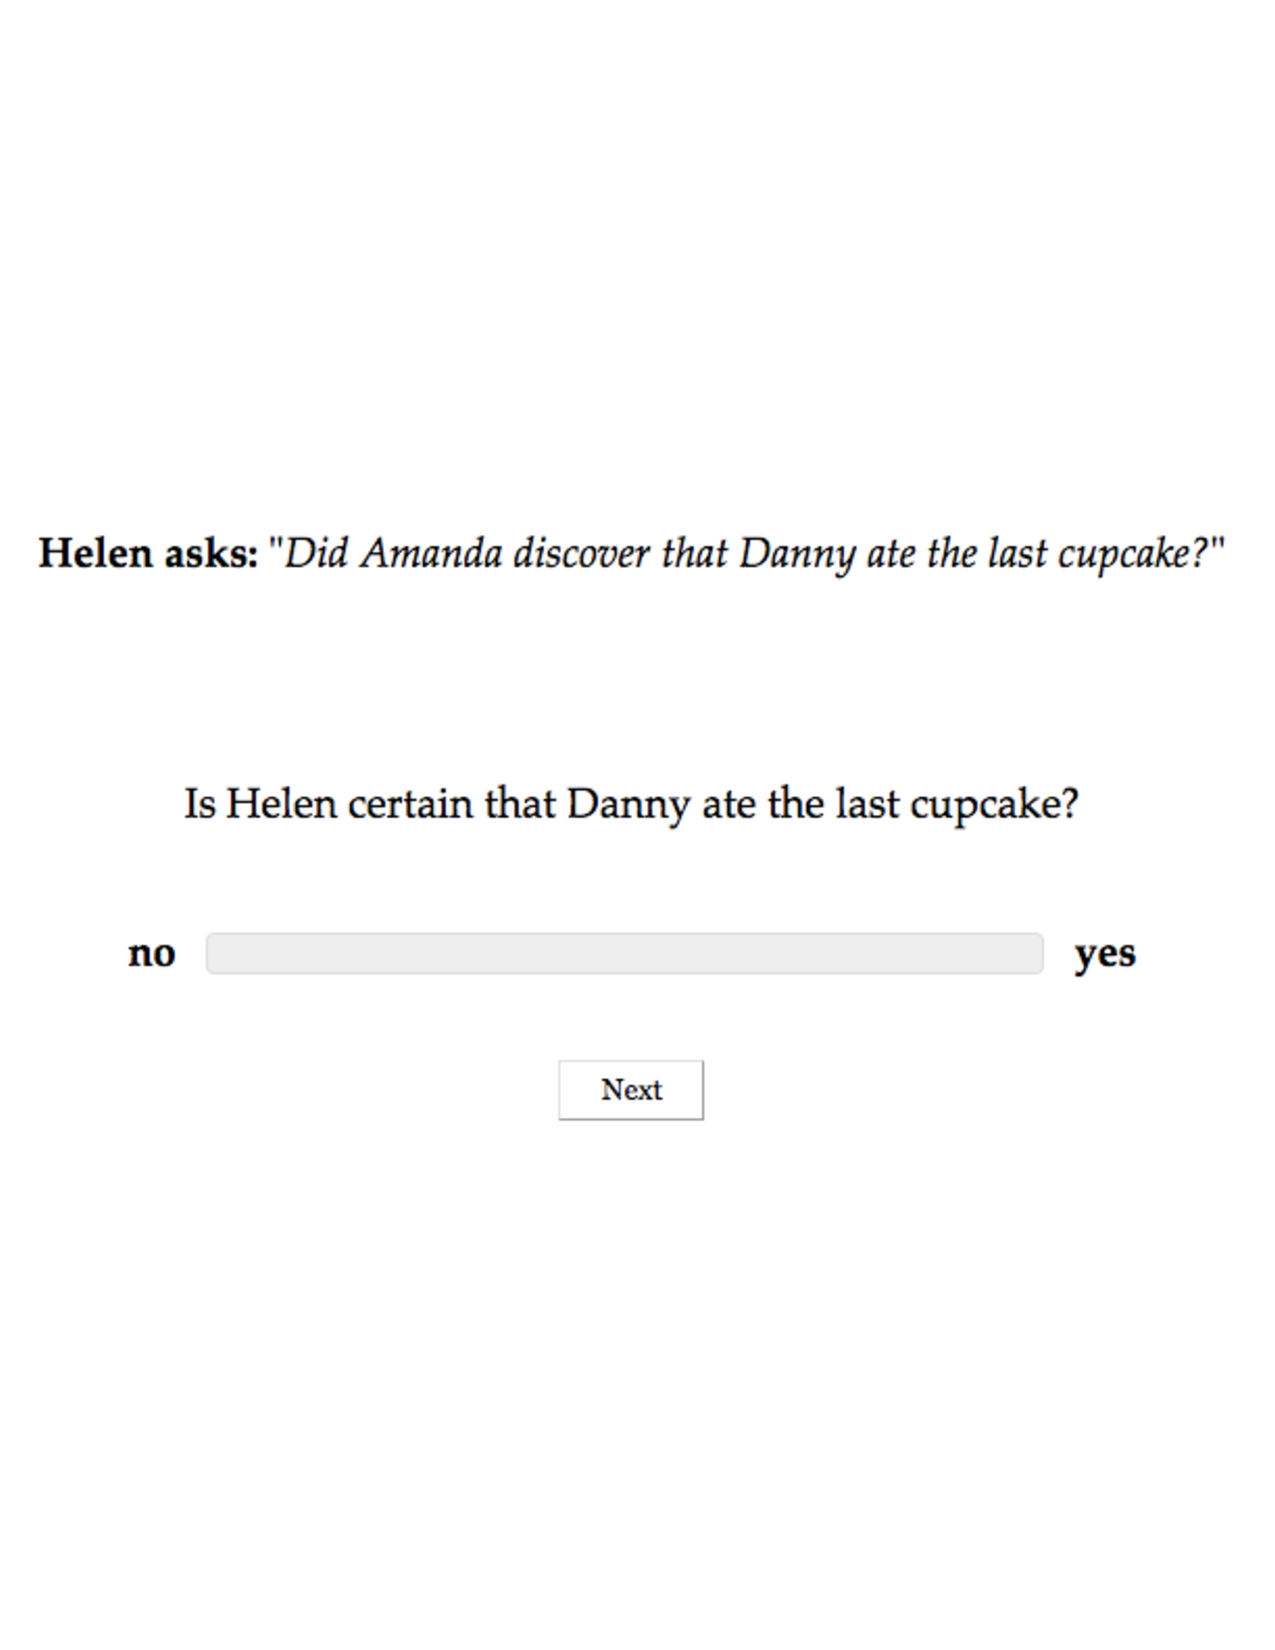
\includegraphics[width=10cm]{figures/trial-exp1}}
\end{center}
\caption{A sample trial in Experiment 1}\label{fig-trial-exp1}
\end{figure}

After completing the experiment, participants filled out a short, optional survey about their age, their gender, their native language(s) and, if English is their native language, whether they are a speaker of American English (as opposed to, e.g., Australian or Indian English). To encourage them to respond truthfully, participants were told that they would be paid no matter what answers they gave in the survey.

\paragraph{Data exclusion}
Prior to analysis, the data from 13 participants who did not self-identify as native speakers of American English were excluded. For the remaining 287 participants, we inspected their responses to the 6 control stimuli, for which we expected low responses because the main clause content is not expected to be projective. As expected, the group mean was low (.14), but the response means of 4 participants were more than 3 standard deviations above the group mean. Closer inspection revealed that these participants' responses to the control stimuli were systematically higher, suggesting that these participants did not attend to the task or interpreted the task differently. The data from these 4 participants were also excluded, resulting in a group mean of .13 on the control stimuli and leaving data from 283 participants (ages 20-71; median: 36; 127 female, 150 male, 2 other).

\subsection{Results}

Each predicate received 283 certainty ratings and each predicate/clause combination received between 5 and 27 ratings (mean: 14.2). The box plot in Figure \ref{f-projectivity} shows the participants' certainty ratings for the target stimuli by predicate, collapsing over complement clauses, as well as the certainty ratings of the main clause control stimuli (abbreviated `MC'). `Factive' predicates are given in darker blue, `veridical non-factive' predicates in lighter blue, `plain non-factive' predicates in brown and `projective non-factive' predicates in black. (This color scheme is used throughout the remainder of the paper.) The mean certainty ratings are given by grey dots and the notches indicate medians. 
%These certainty ratings further support \citetpos{tbd-variability} claim that projectivity is a gradient property of utterance content: the mean certainty ratings of the 21 expressions spread from floor to ceiling, and for many contents there are (non-outlier) certainty ratings from floor to ceiling. 
The mean certainty ratings are consistent with impressionistic judgments reported in the literature: first, the ratings for `factive' predicates are among the highest overall, suggesting high projectivity, and those of `plain non-factive' predicates are among the lowest overall, suggesting low projectivity, with main clause content the least projective; second, the mean certainty ratings of `projective non-factives' are largely higher than those of main clauses and `plain non-factives', which confirms the intuitions of authors like \citet{schlenker10,anand-hacquard2014} and \citet{spector-egre2015} that the content of the complement of some `non-factive' predicates is projective.

\begin{figure}[H]
\centering

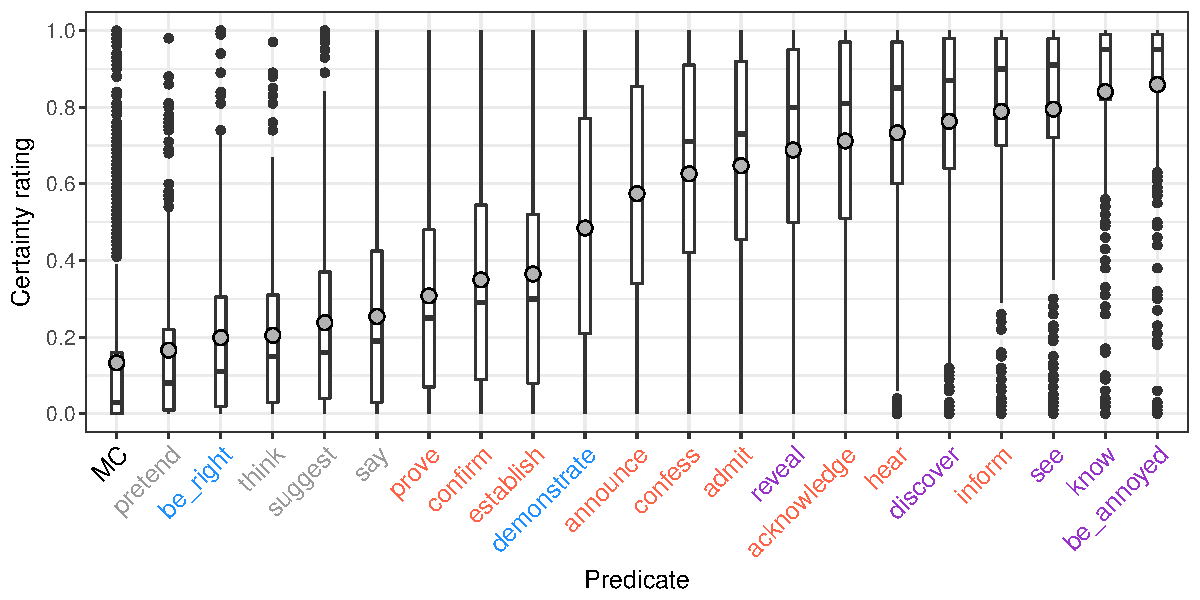
\includegraphics[width=.75\paperwidth]{../results/5-projectivity-no-fact/graphs/boxplot-projectivity}

\caption{Box plot of certainty ratings by predicate, collapsing over complement clauses. Grey dots indicate means and notches indicate medians. `MC' abbreviates main clause controls. `Factive' predicates are given in darker blue, `veridical non-factive' ones in lighter blue, `plain non-factive' ones in brown and `projective non-factive' ones in black. {\bf ADJUST THE COLOR FOR HEAR}}
\label{f-projectivity}
\end{figure}

The certainty ratings plotted in Figure \ref{f-projectivity} also provides further support for \citepos{tbd-variability} claim that projectivity is a gradient property of utterance content. For instance, the mean certainty ratings for the 20 clause-embedding predicates are spread out from .17 for {\em pretend} to .86 for {\em be annoyed}, suggesting gradience in the average extent to which participants took the speakers to be committed to the contents of the complements. Furthermore, for many predicates, the (non-outlier) ratings range from floor to ceiling, suggesting gradience in the extent to which participants took the speakers to be committed to the content of the complement of particular clause-embedding predicates. 

We now address the three research questions about projectivity in (\ref{prq}), repeated below for convenience. 

\begin{exe}
\exi{(\ref{prq})} Research questions about projectivity
\begin{xlist}
\ex How projective is the content of the complement of `factive' predicates?
\ex How projective is the content of the complement of different kinds of `non-factive' predicates?
\ex Does projectivity distinguish `factive' from `non-factive' predicates?
\end{xlist}
\end{exe}


\paragraph{Projectivity of the content of the complement of `factive' predicates}  Like \citet{tbd-variability}, we observe by-predicate and by-participant variability with respect to the projectivity of the contents of the complements of  the 5 `factive' predicates included in Exp.~1. With respect to by-predicate variability, the box plot in Figure \ref{f-projectivity} shows that the mean certainty ratings range from .69 for {\em reveal} to .86 for {\em be annoyed}. Similarly, while the median certainty rating of {\em be annoyed} is at .95, suggesting that half of the participants took the content of the complement to be highly projective, the median certainty rating of {\em reveal} is lower, at .8.
%14 reveal     0.688 0.0362  0.0377 0.652
%17 discover   0.763 0.0328  0.0317 0.730
%19 see        0.795 0.0314  0.0300 0.763
%20 know       0.841 0.0311  0.0263 0.810
%21 be_annoyed 0.859 0.0276  0.0263 0.831
To determine which clause-embedding predicates differed from each other in the projectivity of the content of the  complement, we conducted post hoc pairwise comparisons using Tukey's method (allowing for by-participant variability), using the \verb|lsmeans| package \citep{tukey} in R \citep{r}. We included the main clause controls in the analysis to identify predicates for which the content of the complement was not projective (7358 data points total). The $p$-values for each comparison pair are shown in Table \ref{t-pairwise-proj}. The analysis revealed significant differences among the 5 `factive' predicates: first, the content of the complement of {\em reveal} was significantly less projective than that of the other `factive' predicates; second, the content of the complement of {\em discover} was less projective than that of {\em know} and {\em be annoyed}. These findings align with those of \citealt{tbd-variability}, who also observed that the content of the complement of {\em reveal} was less projective than that of {\em discover}, and that that of {\em discover} was less projective than that of {\em know} and {\em be annoyed}.

The large boxes and the long whiskers for the certainty ratings of the 6 `factive' predicates in Figure \ref{f-projectivity} show that there is by-participant variability. For {\em reveal}, for instance, the median certainty rating was .8, which means that half of the ratings were at or higher than .8 and half of the ratings were at or lower than .8. The box, in turn, shows that the middle 50\% of certainty ratings fell in the range from .5 to .95. The upper whisker shows that the upper 25\% of the ratings fell between .95 and 1, and the lower whisker shows that the lower 25\% of the ratings fell between .5 and 0. Thus, although the content of the complement of {\em reveal} is, on average, quite projective, a quarter of the 283 participants rated the projectivity of the content of the complement above .95, i.e., as highly projective, and another quarter rated it below .5, i.e., as more weakly projective. We also observe from Figure \ref{f-projectivity} that the 5 `factive' predicates may differ in the extent of the by-participant variability. For {\em know} and {\em be annoyed}, the boxes are much smaller and the whiskers much shorter than for the 3 other `factive' predicates, suggesting that there is less by-participant variability for {\em know} and {\em be annoyed} than for the other `factive' predicates. In sum, the by-predicate and by-participant variability suggests that `factive' predicates are heterogeneous with respect to the projectivity of the content of the complement.

\paragraph{Projectivity of the content of the complement of `non-factive' predicates} As discussed in section \ref{s1}, the definition of a `non-factive' predicate in (\ref{def}) means that these predicates are heterogeneous with respect to the projectivity of the content of the complement. Figure \ref{f-projectivity} confirms that there is projection variability between `non-factive' predicates: the mean certainty ratings of the `non-factive' predicates range all the way from from .17 for the `plain non-factive' predicate {\em pretend} to .79 for the `projective non-factive' predicate {\em inform}. However, the projection variability observed between `non-factive' predicates does not align with the distinction between, on the one hand, `plain non-factive' and `veridical non-factive' predicates and, on the other hand, `projective non-factive' predicates. First, pairwise comparison reveals that of the 15 `non-factive' predicates, only the content of the complement of {\em pretend} was indistinguishable in its projectivity from main clause content. This finding means that only the content of the complement of {\em pretend} is not projective and, consequently, that the content of the complement of the remaining 14 `non-factive' predicates, including that of the other 3 `plain non-factive' and the 2 `veridical non-factive' predicates, can be considered projective content, even though some of the contents are only very weakly projective.\footnote{\citet{spector-egre2015} suggested that it is not clear whether the content of the complement of {\em say} is projective (p.1739) but that it is definitely less projective than that of {\em tell}. The findings of Exp.~1 suggest that it is very weakly projective.} Second, for the two `veridical non-factive' predicates, pairwise comparison reveals that the content of the complement of {\em demonstrate} (mean certainty rating: .49) is more projective than that of {\em be right} (mean certainty rating: .2). Thus, these two predicates do not appear to form a natural class with respect to projectivity either. Finally, there is projection variability among the `projective non-factive' predicates: the content of the complement of the 9 `projective non-factive' predicates all differed from one another in projectivity, except for the pairs {\em hear/acknowledge, acknowledge/admit}, {\em admit/announce}, {\em admit/confess}, {\em confess/announce}, {\em establish/confirm} and {\em confirm/prove}. These findings again align with those of \citealt{tbd-variability}, who also observed that the content of the complement of {\em confess} was more projective than that of {\em establish}.\footnote{There are two differences between the findings of Exp.~1 and of \citetpos{tbd-variability} Exps.~1a and 1b. First, the projectivity of the content of the complement of {\em reveal} was significantly higher than that of {\em confess} in their Exp.~1b, but it is only numerically higher in Exp.~1. Second, the certainty ratings were overall higher in \citetpos{tbd-variability} Exps.~1 than in our Exp.~1. For instance, the content of the complement of {\em be annoyed}, which was the most projective in both sets of experiments, received mean certainty ratings of .96  and .92 in their Exps.~1a and 1b, respectively, but only a .86 in our Exp.~1. Similarly, the content of the complement of {\em discover} received mean certainty ratings of .86 and .85 in their Exps.~1a and 1b, respectively, but only a .76 in our Exp.~1. One difference between the two sets of experiments is that \citet{tbd-variability} primarily explored highly projective content whereas our Exp.~1 also included a wide range of less projective content. It is possible that participants' certainty ratings are influenced by the overall projectivity of the contents explored. We leave this matter to future research.} 
In sum, the content of the complement of many `non-factive' predicates is projective, contrary to assumption for `plain non-factive' and `veridical non-factive' predicates, and projection variability is not just observed among `factive' predicates but also among `non-factive' ones.

%Exp 1b: discover $<$ reveal $<$ confess $<$ establish

% Exp 1: discover $<$ reveal, confess $<$ establish, but reveal is not more projective than confess

% 1 MC         0.133 0.00978 0.0100 0.123
% 9 establish  0.365 0.0348  0.0368 0.330
%12 confess    0.626 0.0396  0.0354 0.587
%14 reveal     0.688 0.0362  0.0377 0.652
%17 discover   0.763 0.0328  0.0317 0.730
%20 know       0.841 0.0311  0.0263 0.810
%21 be_annoyed 0.859 0.0276  0.0263 0.831

% Exp 1a
% annoyed       0.9595714 0.01473729 1675.74 0.9306660 0.9884769
% discover      0.8556667 0.01473729 1675.74 0.8267612 0.8845721
% know          0.9233810 0.01473729 1675.74 0.8944755 0.9522864

% Exp 1b
% confessed     0.6869787 0.01499147 1739.4 0.6575755 0.7163819
% discovered    0.8534043 0.01499147 1739.4 0.8240011 0.8828075
% established   0.4177447 0.01499147 1739.4 0.3883415 0.4471479
% is_annoyed    0.9228936 0.01499147 1739.4 0.8934904 0.9522968
% revealed      0.7784255 0.01499147 1739.4 0.7490223 0.8078287
% saw           0.8905957 0.01499147 1739.4 0.8611925 0.9199989



\begin{table}[H]
\setlength\tabcolsep{3pt}

\centering
\small

\begin{tabular}{l l l l l l l l l l l l l l l l l l l l l }
\toprule

& \rot{MC} &   \rot{\color{brown}{\em pretend}\color{black}} & \rot{\color{airforceblue}{\em be right}\color{black}} & \rot{\color{brown}{\em think}\color{black}} &  \rot{\color{brown}{\em suggest}\color{black}} &  \rot{\color{brown}{\em say}\color{black}} & \rot{\color{black}{\em prove}\color{black}} & \rot{{\em confirm}} & \rot{\color{black}{\em establish}\color{black}} & \rot{\color{airforceblue}{\em demonstrate}\color{black}} & \rot{{\em announce}} & \rot{{\em confess}} & \rot{\color{black}{\em admit}\color{black}} & \rot{\color{blue}{\em reveal}\color{black}}  & \rot{{\em acknowledge}}  & \rot{\color{black}{\em hear}\color{black}}  & \rot{\color{blue}{\em discover}\color{black}} & \rot{\color{black}{\em inform}\color{black}}  & \rot{\color{blue}{\em see}\color{black}}  & \rot{\color{blue}{\em know}\color{black}}  \\

\midrule

\color{brown}{\em pretend}\color{black}	&  n.s. & - & - & - & - & - & - & - & - & - & - & - & - & - & - & - & - & - & - \\
\color{airforceblue}{\em be right}\color{black}	& ** & n.s. & - & - & - & - & - & - & - & - & - & - & - & - & - & - & - & - & - & - \\
\color{brown}{\em think}\color{black}		& ** & n.s. & n.s. & - & - & - & - & - & - & - & - & - & - & - & - & - & - & - & - & - \\
\color{brown}{\em suggest}\color{black}	& ***	& . & n.s. & n.s. & - & - & - & - & - & - & - & - & - & - & - & - & - & - & - & - \\
\color{brown}{\em say}	\color{black}	& ***	& ** & n.s. & n.s. & n.s. & - & - & - & - & - & - & - & - & - & - & - & - & - & - & - \\
\color{black}{\em prove}\color{black}		& ***	& *** &  ***  & ** & . & n.s. & - & - & - & - & - & - & - & - & - & - & - & - & - & - \\
\color{black}{\em confirm}\color{black}	&***	& ***  &  ***  &  ***  &  ***  & ** & n.s. & - & - & - & - & - & - & - & - & - & - & - & - & - \\
\color{black}{\em establish}\color{black}	&***	&  ***  &  ***  &  ***  &  ***  &  ***  & n.s & n.s. & - & - & - & - & - & - & - & - & - & - & - & - \\
\color{airforceblue}{\em demonstrate}\color{black} &*** & *** & *** & *** &  *** &  *** &  ***  &  ***  &  ***  & - & - & - & - & - & - & - & - & - & - & - \\
\color{black}{\em announce}\color{black}		& ***	& *** & *** & *** & *** & *** & *** &  ***  &  ***  & ** & - & - & - & - & - & - & - & - & - & - \\
\color{black}{\em confess}\color{black}	& ***	& *** & *** & *** & *** & *** & *** & *** & *** &  ***  & n.s. & - & - & - & - & - & - & - & - & - \\
\color{black}{\em admit}\color{black}		& ***	& *** & *** & *** & *** & *** & *** & *** & *** &  ***  & . & n.s. &  - & - & - & - & - & - & - & - \\
\color{blue}{\em reveal}\color{black}			& ***	& *** & *** & *** & *** & *** & *** & *** & *** &  ***  &  ***  & n.s. & n.s. & - & - & - & - & - & - & - \\
\color{black}{\em acknowledge}\color{black}	& ***	& *** & *** & *** & *** & *** & *** & *** & *** &  ***  &  ***  & ** & n.s. & n.s. & - & - & - & - & - & - \\
\color{black}{\em hear}\color{black}		& ***	& *** & *** & *** & *** & *** & *** & *** & *** & *** &  ***  &  ***  & ** & n.s. & n.s. & - & - & - & - & - \\
\color{blue}{\em discover}\color{black}	& ***		& *** & *** & *** & *** & *** & *** & *** & *** & *** &  ***  &  ***  &  ***  & * & n.s. & n.s. & - & - & - & - \\
\color{black}{\em inform}\color{black}		&***		& *** & *** & *** & *** & *** & *** & *** & *** & *** & *** & *** &  ***  & ** & * & n.s. & n.s. & - & - & - \\
\color{blue}{\em see}\color{black}		&***		& *** & *** & *** & *** & *** & *** & *** & *** & *** & *** &  ***  &  ***  &  ***  & ** & n.s. & n.s. & n.s. & - & - \\
\color{blue}{\em know}\color{black}		&***		& *** & *** & *** & *** & *** & *** & *** & *** & *** & *** & *** & *** & *** & *** & *** & * & n.s. & n.s. & -  \\
\color{blue}{\em be annoyed}\color{black}	&***		& *** & *** & *** & *** & *** & *** & *** & *** & ***  & ***  & *** & *** & *** & *** & *** & ** & . & n.s. & ns  \\

\bottomrule
\end{tabular}
\caption{P-values associated with pairwise comparison of certainty ratings of the 20 clause-embedding predicates and the main clause controls using Tukey's method. `***' indicates significance at .0001, `**' at .01, `*' at .05, `.' marginal significance at .1, and `n.s' indicates no significant difference in means. `MC' abbreviates main clause controls. `Factive' predicates are given in darker blue, `veridical non-factive' ones in lighter blue, `plain non-factive' ones in brown and `projective non-factive' ones in black.}\label{t-pairwise-proj}
\end{table} 

\paragraph{Distinguishing `factive' and `non-factive' predicates by projectivity} Having established that the content of the complement of both `factive' and `non-factive' predicates is projective, albeit to varying degrees, we now turn to the research question in (\ref{prq}c), whether projectivity distinguishes `factive' from `non-factive' predicates. Although `factive' predicates received some of the highest certainty ratings, there are `non-factive' predicates, specifically `projective non-factive' predicates, that also received high ratings. For instance, the mean certainty ratings of the `projecting non-factive' predicates {\em acknowledge} (.71) and {\em admit} (.65) are close to that of the `factive' predicate {\em reveal} (.69). Further, the mean certainty rating of the `projecting non-factive' predicate {\em inform} (.79) is close to that of the `factive' predicate {\em see} (.8) and higher than that of the `factive' predicates {\em reveal} and  {\em discover} (.76).  In fact, pairwise comparison (see Table \ref{t-pairwise-proj}) shows that the projectivity of the content of the complement of some `projective non-factive' predicates is indistinguishable from that of `factive' predicates. Specifically, the projectivity of the content of the complement of the `projective non-factive' predicate {\em inform} is indistinguishable from that of the `factive' predicates {\em know, be annoyed} and {\em see}, that of the `projective non-factive' predicate {\em hear} is indistinguishable from that of the `factive' predicates {\em reveal, discover} and {\em see}, that of the `projective non-factive' predicate {\em acknowledge} is indistinguishable from that of the `factive' predicate {\em discover}, and that of the `projective non-factive' predicates {\em confess} and {\em admit} is indistinguishable from that of the `factive' predicate {\em reveal}. These findings suggest that the projectivity of the content of the complement of the 5 `factive' predicates under investigation is not categorically higher of that of the `projective non-factive' predicates {\em inform, hear, acknowledge, confess} and {\em admit}. In other words, although the content of the complement of `factive' predicates tends to be more projective than that of `non-factive' predicates, projectivity does not categorically distinguish `factive' from `non-factive' predicates.


%  verb        Mean   CILow CIHigh  YMin
%   <fct>      <dbl>   <dbl>  <dbl> <dbl>
% 1 MC         0.133 0.00978 0.0100 0.123
% 2 pretend    0.166 0.0238  0.0255 0.142
% 3 be_right   0.199 0.0282  0.0305 0.170
% 4 think      0.205 0.0232  0.0249 0.182
% 5 suggest    0.238 0.0285  0.0285 0.209
% 6 say        0.254 0.0302  0.0324 0.224
% 7 prove      0.308 0.0293  0.0289 0.279
% 8 confirm    0.350 0.0321  0.0335 0.318
% 9 establish  0.365 0.0348  0.0368 0.330
%10 demonstra? 0.485 0.0384  0.0369 0.446
%11 announce   0.575 0.0361  0.0375 0.539
%12 confess    0.626 0.0396  0.0354 0.587
%13 admit      0.647 0.0376  0.0347 0.610
%14 reveal     0.688 0.0362  0.0377 0.652
%15 acknowled? 0.712 0.0341  0.0328 0.678
%16 hear       0.733 0.0349  0.0340 0.698
%17 discover   0.763 0.0328  0.0317 0.730
%18 inform     0.789 0.0347  0.0289 0.754
%19 see        0.795 0.0314  0.0300 0.763
%20 know       0.841 0.0311  0.0263 0.810
%21 be_annoyed 0.859 0.0276  0.0263 0.831

%  verb        Median Quantile1 Quantile2 Quantile4 Quantile5
% 1 acknowledge  0.81       1        0.97      0.51          0
% 2 admit        0.73       1        0.92      0.455         0
% 3 announce     0.580      1        0.855     0.34          0
% 4 be_annoyed   0.95       1        0.99      0.85          0
% 5 be_right     0.11       1        0.305     0.02          0
% 6 confess      0.71       1        0.91      0.42          0
% 7 confirm      0.290      1        0.545     0.09          0
% 8 MC           0.03       1        0.16      0             0
% 9 demonstrate  0.49       1        0.77      0.21          0
%10 discover     0.87       1        0.98      0.64          0
%11 establish    0.3        1        0.52      0.08          0
%12 hear         0.85       1        0.97      0.6           0
%13 inform       0.9        1        0.98      0.7           0
%14 know         0.95       1        0.99      0.82          0
%15 pretend      0.08       0.98     0.22      0.01          0
%16 prove        0.25       1        0.48      0.07          0
%17 reveal       0.8        1        0.95      0.5           0
%18 say          0.19       1        0.425     0.03          0
%19 see          0.91       1        0.98      0.72          0
%20 suggest      0.16       1        0.37      0.04          0
%21 think        0.15       0.97     0.31      0.03          0
 

\subsection{Discussion}

Exp.~1 expanded on \citetpos{tbd-variability} experiments in exploring the projectivity of the content of the complement of 20 `factive' and `non-factive' clause-embedding predicates. This experiment confirmed 
\citepos{tbd-variability} finding that there is projection variability among `factive' predicates and that projectivity is a gradient property of utterance content. Exp.~1 also confirmed the intuitions of semanticists that the content of the complement of many `non-factive' predicates, dubbed `projective non-factive' predicates here, is projective, albeit to varying degrees. In fact, pairwise comparison of the content of the complement of the 20 clause-embedding predicates with non-projective main clause content revealed that the content of the complement of all predicates except for {\em pretend} was projective, even though some was only very weakly projective. This finding identifies a lacuna in projection analyses because, as discussed in section \ref{s1}, currently available projection analyses are limited to `factive' predicates. 

The findings of Exp.~1 also showed that projectivity does not categorically distinguish `factive' and `non-factive' predicates: this is primarily due the projection variability between `factive' predicates and the fact that the projectivity of many `projective non-factive' predicates is as high as that of `factive' predicates. It is important to note that, by the definition of `factive' and `non-factive' predicates in (\ref{def}), projectivity alone is not assumed to distinguish the two classes of predicates. Rather, `factive' predicates differ from `non-factive' ones in that the content of the complement of the former is both projective and entailed. The finding of Exp.~1 that projectivity alone indeed does not categorically distinguish `factive' from `non-factive' predicates underlines the importance of entailment in distinguishing `factive' and `non-factive' predicates. The experiments described in the next section were designed to explore whether the content of the clausal complement of the same 20 clause-embedding predicates is entailed, to identify whether there is a categorical distinction between `factive' and `non-factive' predicates. 

\section{Experiment 2: Entailment}\label{s3}

The two experiments described in this section were designed explore whether the content of the clausal complement is entailed by the content of unembedded matrix sentences with the 20 clause-embedding predicates. Given the standard definition of the entailment relation, it is straightforward to establish that the content of a natural language sentence $\phi$ does not entail the content of a natural language sentence $\psi$, namely by pointing to a world in which the content of $\phi$ is true and the content of $\psi$ is false. It is also relatively straightforward to argue that the content of a sentence $\phi$ entails the content of a sentence $\psi$ if the content of some expression in $\phi$ denotes a subset of the content of some expression in $\psi$. For instance, in the example in (\ref{ent1}a),  the content of $\phi$ entails the content of $\psi$ because the denotation of {\em black cat} in $\phi$ is a subset of the denotation of {\em cat} in $\psi$. By contrast, in the example in (\ref{ent1}b), the two sentences $\phi$ and $\psi$ do not stand in such a structural relationship that would allow one to argue that the content of $\phi$ entails the content of $\psi$. It is also impossible to empirically verify that the content of $\phi$ entails the content of $\psi$ in (\ref{ent1}b) because it is impossible to  verify that $\psi$ is true in all worlds in which $\phi$ is true. 

\begin{exe}
\ex\label{ent1}
\begin{xlist}
\ex $\phi$: Sam owns a black cat. \hspace*{1.5cm} $\psi$: Sam owns a cat.

\ex $\phi$: Sam knows that it's raining. \hspace*{.6cm} $\psi$: It's raining.

\end{xlist}
\end{exe}
To establish whether the content of unembedded matrix sentences with a clause-embedding predicate entails the content of the clausal complement, linguists rely on diagnostics that are taken to provide evidence for an entailment relationship. Two standard diagnostics, which were already applied to sentences with the emotive predicate {\em regret} in section \ref{s1}, are given in (\ref{diag}). Under the `inference diagnostic' in (\ref{diag}a), the content of an unembedded matrix sentence with a clause-embedding predicate entails the content of the complement if and only if the content of the complement definitely follows from true statements of the unembedded matrix sentence. Under the `contradictoriness diagnostic' in (\ref{diag}b), such an entailment relationship holds if and only utterances of the unembedded matrix sentence that are followed by a denial of the content of the complement are contradictory. 

\begin{exe}
\ex\label{diag} Two diagnostics for entailment \hfill (see also \citealt[\S3.1]{ccmg90})
\begin{xlist}
\ex  Inference diagnostic \\ $\phi$ entails $\psi$ if and only if, if $\phi$ is true, then (the truth of) $\psi$ definitely follows. 

\ex  Contradictoriness diagnostic \\ $\phi$ entails $\psi$ if and only if sentences of the form {\em A and not B} are contradictory. 

\end{xlist}
\end{exe}
These two diagnostics for entailment are applied to the content of the complement of the 20 clause-embedding predicates in Exps.~2a and 2b, respectively. We present the findings of the two experiments in sections \ref{s31} and \ref{s32}, and then discuss the findings jointly in section \ref{s33}.

\subsection{Experiment 2a: Inference diagnostic for entailment}\label{s31}

This experiment explored whether the content of the clausal complement of the 20 clause-embedding predicates is an entailment based on the inference diagnostic for entailment in (\ref{diag}a). In contrast to the entailment relationship, which is binary and categorical, the inference relationship between the contents of two sentences $\phi$ and $\psi$ is gradient: given a true statement $\phi$, the truth of $\psi$ follows to varying degrees. To illustrate, assume that Chris wears his pajamas whenever he is at home and that he doesn't wear pajamas outside of his home. Now consider the contents of the sentences $\phi_1$ to $\phi_5$ in (\ref{chris}). The (truth of the) content of the statement $\psi$ {\em Chris is wearing his pajamas} definitely follows from a true statement of $\phi_1$, it follows to increasingly lower degrees from true statements of $\phi_2$ to $\phi_4$ and it definitely does not follow from a true statement of $\phi_5$. 

\begin{exe}
\ex\label{chris}
\begin{xlist}
\exi{$\phi_1$} Chris is at home.
\exi{$\phi_2$} Chris is likely at home.
\exi{$\phi_3$} Chris is possibly at home.
\exi{$\phi_4$} There is a slight possibility that Chris is at home.
\exi{$\phi_5$} Chris is not at home.
\end{xlist}
\end{exe}

In applying the inference diagnostic for entailment in Exp.~2a, we assume that if the content of $\phi$ entails the content of $\psi$, then the (truth of the) content of $\psi$ definitely follows from true statements of $\phi$, i.e., the strength of the inference is at ceiling. If the content of $\phi$ does not entail the content of $\psi$, then the strength of the inference is anywhere below ceiling. Exp.~2a investigated the strength of the inference from true statements of unembedded matrix sentences with the 20 clause-embedding predicates to the content of the clausal complements by collecting gradient inference ratings.

\subsubsection{Methods}

\paragraph{Participants} 300 participants with U.S.\ IP addresses and at least 99\% of previous HITs approved were recruited on Amazon's Mechanical Turk platform (ages: 19-69, median: 36; 152 female, 148 male). They were paid 75 cents for participating in the experiment.

\paragraph{Materials} The target stimuli were 400 unembedded matrix sentences that were constructed by combining the 400 predicate/clause combinations of Exp.~1 with a random proper name subject whose gender differed from the gender of the proper name subject of the embedded clause. As illustrated in the sample stimuli in (\ref{stims2}), these matrix sentences were presented to participants as true statements. For each of the 400 target stimuli, the inference that was tested was the inference to the content of the clausal complement: for instance, participants were asked about (\ref{stims2}a) whether it follows that Danny ate the last cupcake and about (\ref{stims2}b) whether it follows that Emma studied on Saturday morning.

\begin{exe}
\ex\label{stims2}
\begin{xlist}
\ex {\bf What is true:} Melissa knows that Danny ate the last cupcake.
%\\ Does it follow that Danny ate the last cupcake?
\ex {\bf What is true:} Jerry pretended that Emma studied on Saturday morning.
%\\ Does it follow that Emma studied on Saturday morning?
\end{xlist}
\end{exe}

The experiment also included eight control stimuli, which were used to assess whether participants attended to the task and whether they interpreted the task correctly. For the four control stimuli in (\ref{control-good2}), the tested inferences are lexical entailment of the true statements: for instance, that Frederick solved the problem is a lexical entailment of the true statement that Frederick managed to solve the problem. Because the tested inferences for these four control stimuli are lexical entailments, we expected the inference ratings to be at ceiling. In contrast, the inferences tested with the four control stimuli in (\ref{control-bad2}) definitely do not follow from these true statements: in (\ref{control-bad2}a), that Dana wears a wig does not follow from Dana watching a movie last night, and that Madison closed the window is the negation of what actually follows from the true statement in (\ref{control-bad2}c). We expected the inference ratings for these four control stimuli to be at floor.

\begin{exe}
\ex\label{control-good2}
\begin{xlist}
\ex {\bf What is true:} Zack bought himself a car this morning. (Tested inference: Zack owns a car.)
\ex {\bf What is true:} Tara broke the window with a bat. (Tested inference: The window broke.)
\ex {\bf What is true:} Frederick managed to solve the problem. (Tested inference: Frederick solved the problem.)
\ex {\bf What is true:} Vanessa happened to look into the mirror. (Tested inference: Vanessa looked into the mirror.)
\end{xlist}
\ex\label{control-bad2}
\begin{xlist}
\ex {\bf What is true:} Dana watched a movie last night. (Tested inference: Dana wears a wig.)
\ex {\bf What is true:} Hendrick is renting an apartment. (Tested inference: The apartment has a balcony.)
\ex {\bf What is true:} Madison was unsuccessful in closing the window. (Tested inference:  Madison closed the window.)
\ex {\bf What is true:} Sebastian failed the exam. (Tested inference: Sebastian did really well on the exam.)
\end{xlist}
\end{exe}

Each participant saw a random set of 28 stimuli: each set contained one target stimulus for each of the 20 predicates (each with a unique complement clause) and the same 8 control stimuli. Trial order was randomized.

\paragraph{Procedure} Participants were told that they would read true statements and that they would be asked to assess whether a second statement follows from the first, true statement. On each trial, participants read the true statement and were asked to respond to the question {\em Does it follow that\ldots} where the continuation was realized by the complement of the clause-embedding predicate. Participants gave their responses on a sliding scale from `definitely doesn't follow' (coded as 0) to `definitely follows' (coded as 1), as shown in Figure \ref{f-trial-exp3}.

\begin{figure}[H]
\begin{center}
\fbox{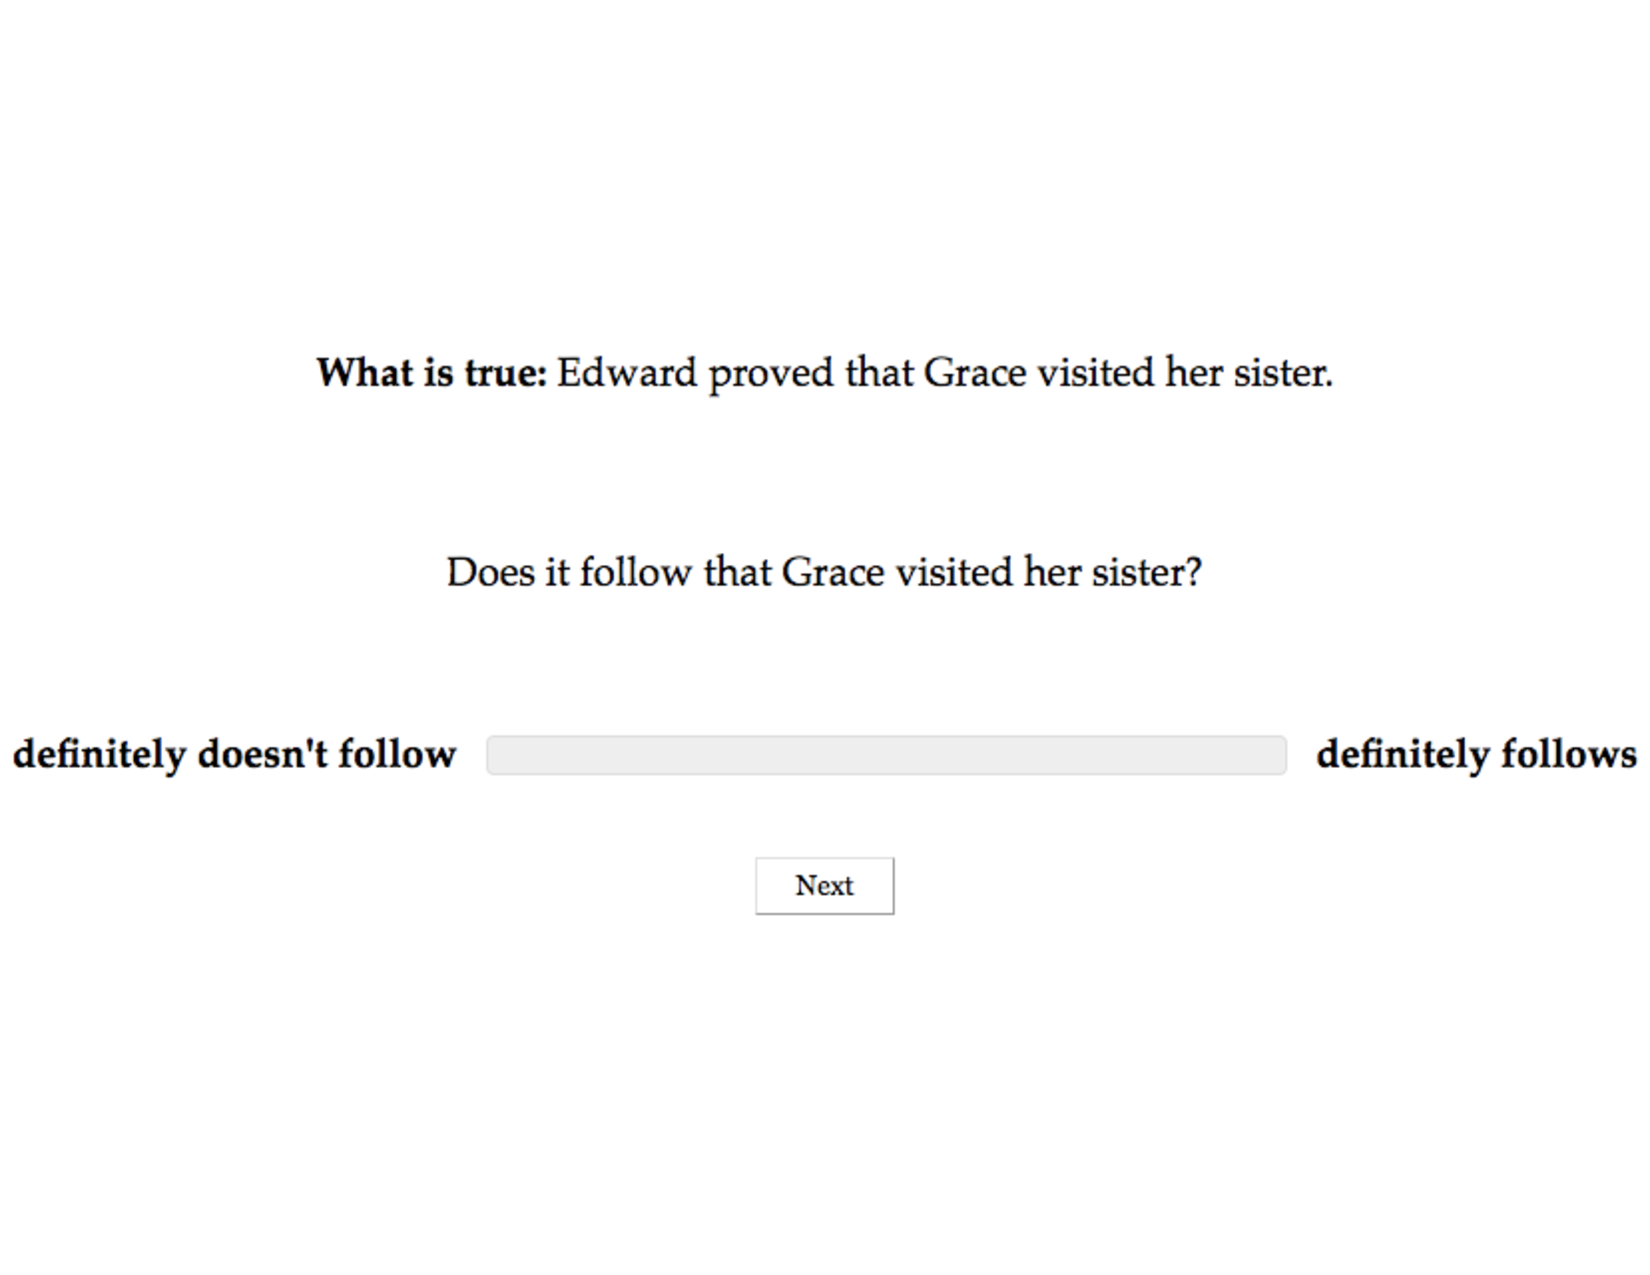
\includegraphics[width=13cm]{figures/inference-trial}}
\end{center}
\caption{A sample trial in Experiment 2a}\label{f-trial-exp3}
\end{figure}

To familiarize participants with the task, they first responded to the two familiarization stimuli in (\ref{train2}), where the inference tested was the inference to the content of the clausal complement. Participants who rated (\ref{train2}a) in the lower half of the sliding scale or (\ref{train2}b) in the upper half of the sliding scale were given an explanation for why their answer was wrong. Participants could only advance to the 28 stimuli if they gave a plausible rating to the two familiarization stimuli, i.e., a rating in the upper half of the sliding scale for (\ref{train2}a) and in the lower half for (\ref{train2}b).

\begin{exe}
\ex\label{train2}
\begin{xlist}
\ex {\bf What is true:} Drew is correct that Patty lives in Canada. 

\ex {\bf What is true}: Drew believes that Patty lives in Canada.
\end{xlist}
\end{exe}

After responding to the 28 stimuli, participants filled out a short, optional survey about their age, their gender, their native language(s) and, if English is their native language, whether they are a speaker of American English (as opposed to, e.g., Australian or Indian English). To encourage them to respond truthfully, participants were told that they would be paid no matter what answers they gave in the survey.

\paragraph{Data exclusion}

Prior to analysis, the data from 14 participants who did not self-identify as native speakers of American English were excluded. For the remaining 286 participants, we inspected their responses to the 8 control stimuli. The group means for the four control stimuli in (\ref{control-good2}) where the inference to the content of the clausal complement was expected to follow was .94 and the group mean for the four control stimuli in (\ref{control-bad2}) where the inference to the content of the clausal complement was expected to not follow was .05. These group means suggest that, overall, participants attended to and understood the task. The response means of 7 participants were more than 3 standard deviations below the group mean for the control stimuli in (\ref{control-good2}) or above the group mean for the control stimuli in (\ref{control-bad2}). Closer inspection revealed that these participants' responses to the control stimuli were systematically higher or lower, respectively, suggesting that these participants did not attend to the task or interpreted the task differently. The data from these 7 participants were also excluded, leaving data from 279 participants (ages 19-69; median: 36; 142 female, 137 male) and resulting in new group means of .95 for the control stimuli in (\ref{control-good2}) and .04 for the control stimuli in (\ref{control-bad2}).

\subsubsection{Results}

Each of the 20 clause-embedding predicates received 279 ratings and each of the 400 predicate/clause combinations received between 5 and 24 ratings (mean: 13.9). The box plot in Figure \ref{f-veridicality-predicate2} shows participants' inference ratings by predicate, collapsing over the 20 complement clauses. The `plain non-factive' predicates {\em pretend, think, suggest} and {\em say} received among the lowest ratings overall, as expected from the assumption that the content of the complement of these predicates is not entailed. Only the mean inference rating for {\em pretend} (.12) came close to the mean inference rating for the non-entailing control stimuli in (\ref{control-bad2}) (which was .04). The mean inference ratings for the other `plain non-factive' predicates were higher, at .31 for {\em think}, .34 for {\em suggest} and .68 for {\em say}. The mean inference ratings of several predicates were at or close to ceiling (recall the group mean of .95 for the control stimuli in (\ref{control-good2})), including the `factive' predicates {\em see} (.94), {\em discover} (.94),  {\em know} (.93) and {\em be annoyed} (.92), as well as the `veridical non-factive' predicate {\em be right} (.95), but also the `projective non-factive' predicates {\em prove} (.95),  {\em establish} (.90), {\em admit} (.90), and {\em acknowledge} (.90). This finding suggests that participants took the truth of the content of the clausal complement of these predicates to (mostly) follow from the true statements of unembedded matrix sentences with these predicates. However, for the `factive' predicate {\em reveal}, the larger box and longer lower whisker already suggest that there were participants for whom the content of the clausal complement of this predicate did not follow strongly from true statements with this predicate. The same holds for the purported `veridical non-factive' predicate {\em demonstrate}, whose mean inference rating was not at ceiling (.84). We also note that the inference ratings for the `projective non-factive' predicate {\em hear} were quite low, suggesting, as discussed in section \ref{s2}, that participants indeed interpreted the target stimuli with {\em hear} using the evidential sense of {\em hear}, not the sensory sense of {\em hear}. 

%          verb      Mean       YMin      YMax
%1  acknowledge 0.8980287 0.87993817 0.9159525
%2        admit 0.8984946 0.88035663 0.9165950
%3     announce 0.8034409 0.77417742 0.8306201
%4   be_annoyed 0.9150896 0.89709409 0.9314023
%5     be_right 0.9472043 0.93537455 0.9581362
%6      confess 0.8837993 0.86551523 0.9022661
%7      confirm 0.9361290 0.92328853 0.9485726
%8  demonstrate 0.8428674 0.81867204 0.8683889
%9     discover 0.9394624 0.92898835 0.9494991
%10   establish 0.8989247 0.88118100 0.9168486
%11        hear 0.4996057 0.46280108 0.5363100
%12      inform 0.8301434 0.80379301 0.8570609
%13        know 0.9251613 0.91092563 0.9387849
%14     pretend 0.1219713 0.09496774 0.1505968
%15       prove 0.9492832 0.93799194 0.9594292
%16      reveal 0.8963082 0.87770520 0.9145878
%17         say 0.6786022 0.64214785 0.7137796
%18         see 0.9426523 0.93217921 0.9526900
%19     suggest 0.3413262 0.30690950 0.3740600
%20       think 0.3138351 0.28154032 0.3453790

\begin{figure}[h!]
\centering

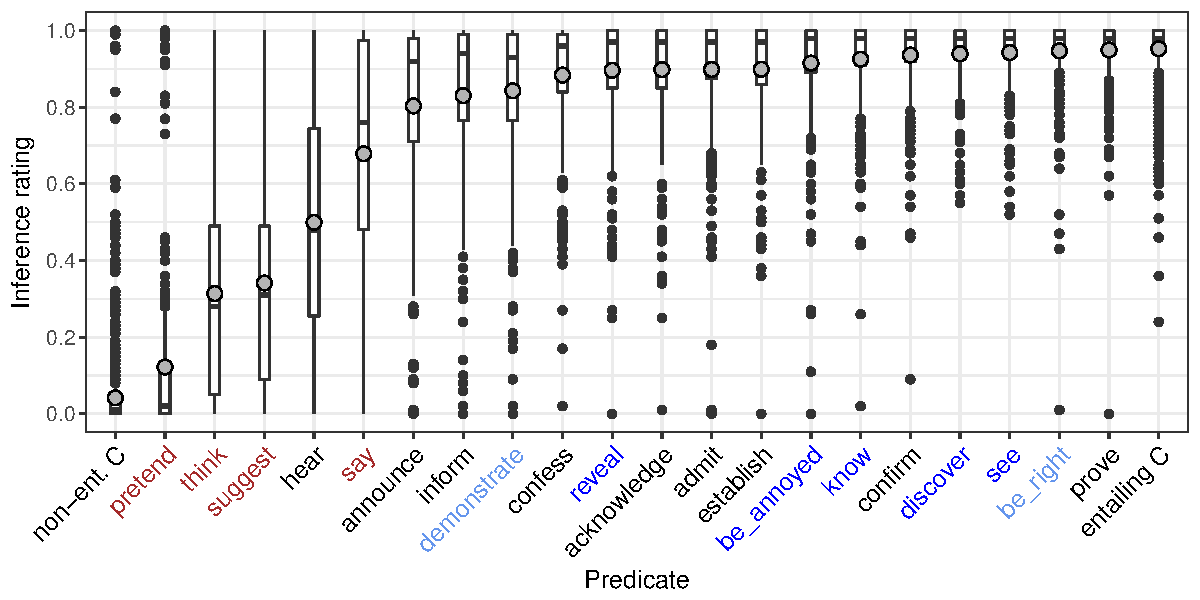
\includegraphics[width=.75\paperwidth]{../results/4-veridicality3/graphs/boxplot-inference}

\caption{Box plot of inference ratings by predicate, collapsing across complement clauses. Grey dots indicate means and notches indicate medians. `Factive' predicates are given in darker blue, `veridical non-factive' ones in lighter blue, `plain non-factive' ones in brown and `projective non-factive' ones in black. {\bf FIX COLOR OF HEAR}}
\label{f-veridicality-predicate2}
\end{figure}

To determine which clause-embedding predicates differed from each other in the strength of the inference to the content of the  complement, we conducted post hoc pairwise comparisons using Tukey's method (allowing for by-participant variability), using the \verb|lsmeans| package \citep{tukey} in R \citep{r}. We included the control stimuli in (\ref{control-good2}) in the analysis to identify predicates for which the inference to the content of the complement was at ceiling (6696 data points total). The $p$-values for each comparison pair are shown in Table  \ref{t-pairwise2}. These results suggest no difference in the strength of the inference to the content of the controls in (\ref{control-good2}) and the content of the complement of the `factive' predicates {\em see, discover, know} and {\em be annoyed}, of the `veridical non-factive' predicate {\em be right} and the `projective non-factive' predicates {\em prove} and {\em confirm}. These findings support an analysis of the content of the complement of these expressions as an entailment.  {\bf DO WE WANT TO INCLUDE THE CONTROLS? RESULTS CHANGE}

\begin{table}[h!]
\setlength\tabcolsep{3pt}

\centering
\small

\begin{tabular}{l l l l l l l l l l l l l l l l l l l l l }
\toprule

 &  \rot{\color{brown}{\em pretend}\color{black}} & \rot{\color{brown}{\em think}\color{black}} & \rot{\color{brown}{\em suggest}\color{black}} &  \rot{\color{black}{\em hear}\color{black}} &  \rot{\color{brown}{\em say}\color{black}} & \rot{{\em announce}} & \rot{{\em inform}} & \rot{\color{airforceblue}{\em demonstrate}\color{black}} & \rot{\color{black}{\em confess}\color{black}} & \rot{\color{blue}{\em reveal}\color{black}} & \rot{{\em acknowledge}} & \rot{{\em admit}} & \rot{\color{black}{\em establish}\color{black}}  & \rot{\color{blue}{\em be annoyed}\color{black}}  & \rot{\color{blue}{\em know}\color{black}}  & \rot{\color{black}{\em confirm}\color{black}} & \rot{\color{blue}{\em discover}\color{black}}  & \rot{\color{blue}{\em see}\color{black}}  & \rot{\color{airforceblue}{\em be right}\color{black}} & \rot{\color{black}{\em prove} \color{black}}  \\
\midrule

\color{brown}{\em think}\color{black}		& *** & - & - & - & - & - & - & - & - & - & - & - & - & - & - & - & - & - & - & -\\
\color{brown}{\em suggest}\color{black}			& *** & n.s. & - & - & - & - & - & - & - & - & - & - & - & - & - & - & - & - & - & - \\
\color{black}{\em hear}	\color{black}		& *** & *** & *** & - & - & - & - & - & - & - & - & - & - & - & - & - & - & - & - & -\\
\color{brown}{\em say}\color{black}		& *** & *** & *** & *** & - & - & - & - & - & - & - & - & - & - & - & - & - & - & - & -\\
\color{black}{\em announce}\color{black}		& *** & *** & *** & *** & *** & - & - & - & - & - & - & - & - & - & - & - & - & - & - & -\\
\color{black}{\em inform}\color{black}		& *** & *** & *** & *** & *** & n.s. & - & - & - & - & - & - & - & - & - & - & - & - & - & -\\
\color{airforceblue}{\em demonstrate}\color{black}		& *** & *** & *** & *** & *** & n.s. & n.s. & - & - & - & - & - & - & - & - & - & - & - & - & -\\
\color{black}{\em confess}\color{black}		& *** & *** & *** & *** & *** & *** & * & n.s. & - & - & - & - & - & - & - & - & - & - & - & -\\
\color{blue}{\em reveal}\color{black}		& *** & *** & *** & *** & *** & *** & ** & * & n.s. & - & - & - & - & - & - & - & - & - & - & -\\
\color{black}{\em acknowledge}\color{black}	& *** & *** & *** & *** & *** & *** & ** & * & n.s. & n.s. & - & - & - & - & - & - & - & - & - & -\\
\color{black}{\em admit}\color{black}			& *** & *** & *** & *** & *** & *** & ** & * & n.s. & n.s. & n.s. & - & - & - & - & - & - & - & - & -\\
\color{black}{\em establish}\color{black}		& *** & *** & *** & *** & *** & *** & ** & * & n.s. & n.s. & n.s. &  ns & - & - & - & - & - & - & - & -\\
\color{blue}{\em be annoyed}\color{black}	& *** & *** & *** & *** & *** & *** & *** & ** & n.s. & n.s. & n.s. & n.s. & n.s. & - & - & - & - & - & - & -\\
\color{blue}{\em know}\color{black}		& *** & *** & *** & *** & *** & *** & *** & *** & n.s. & n.s. & n.s. & n.s. & n.s. & n.s. & - & - & - & - & - & -\\
\color{black}{\em confirm}\color{black}		& *** & *** & *** & *** & *** & *** & *** & *** & * & n.s. & n.s. & n.s. & n.s. & n.s. & n.s. & - & - & - & - & -\\
\color{blue}{\em discover}\color{black}			& *** & *** & *** & *** & *** & *** & *** & *** & * & n.s. & n.s. & n.s. & n.s. & n.s. & n.s. & n.s. & - & - & - & -\\
\color{blue}{\em see}\color{black}			& *** & *** & *** & *** & *** & *** & *** & *** & ** & n.s. & n.s. & n.s. & n.s. & n.s. & n.s. & n.s. & n.s. & - & - & - \\
\color{airforceblue}{\em be right}\color{black}			& *** & *** & *** & *** & *** & *** & *** & *** & ** & * & . & . & . & n.s. & n.s. & n.s. & n.s. & n.s. & - & - \\
\color{black}{\em prove}\color{black}		& *** & *** & *** & *** & *** & *** & *** & *** & **  & *  & * & * & * & n.s. & n.s. & n.s. & n.s. & n.s. & n.s. & - \\
\color{black}controls (\ref{control-good2})\color{black}		& *** & *** & *** & *** & *** & *** & *** & *** & ***  & ** & ** & ** & ** & . & n.s. & n.s. & n.s. & n.s. & n.s.  & n.s. \\

\bottomrule
\end{tabular}
\caption{P-values associated with pairwise comparison of inference ratings of the 20 clause-embedding predicates and the controls in (\ref{control-good2}) using Tukey's method. `***' indicates significance at .0001, `**' at .01, `*' at .05, `.' marginal significance at .1, and `n.s.' indicates no significant difference in means. `Factive' predicates are given in darker blue, `veridical non-factive' ones in lighter blue, `non-factive' ones in brown and `apparently factive' ones in black.}\label{t-pairwise2}
\end{table}

%\begin{table}[h!]
%\setlength\tabcolsep{3pt}
%
%\centering
%\small
%
%\begin{tabular}{l l l l l l l l l l l l l l l l l l l l }
%\toprule
%
% &   \rot{\color{black}controls\color{black}}  & \rot{\color{brown}{\em pretend}\color{black}} & \rot{\color{brown}{\em think}\color{black}} & \rot{\color{brown}{\em suggest}\color{black}} &  \rot{\color{blue}{\em hear}\color{black}} &  \rot{\color{brown}{\em say}\color{black}} & \rot{{\em announce}} & \rot{{\em inform}} & \rot{\color{airforceblue}{\em demonstrate}\color{black}} & \rot{\color{black}{\em confess}\color{black}} & \rot{\color{blue}{\em reveal}\color{black}} & \rot{{\em acknowledge}} & \rot{{\em admit}} & \rot{\color{black}{\em establish}\color{black}}  & \rot{\color{blue}{\em be annoyed}\color{black}}  & \rot{\color{blue}{\em know}\color{black}}  & \rot{\color{black}{\em confirm}\color{black}} & \rot{\color{blue}{\em discover}\color{black}}  & \rot{\color{blue}{\em see}\color{black}}  & \rot{\color{airforceblue}{\em be right}\color{black}} \\
%\midrule
%
%\color{brown}{\em think}\color{black}		& *** & - & - & - & - & - & - & - & - & - & - & - & - & - & - & - & - & - & - \\
%\color{brown}{\em suggest}\color{black}			& *** & n.s. & - & - & - & - & - & - & - & - & - & - & - & - & - & - & - & - & - \\
%\color{blue}{\em hear}	\color{black}		& *** & *** & *** & - & - & - & - & - & - & - & - & - & - & - & - & - & - & - & - \\
%\color{brown}{\em say}\color{black}		& *** & *** & *** & *** & - & - & - & - & - & - & - & - & - & - & - & - & - & - & - \\
%\color{black}{\em announce}\color{black}		& *** & *** & *** & *** & *** & - & - & - & - & - & - & - & - & - & - & - & - & - & - \\
%\color{black}{\em inform}\color{black}		& *** & *** & *** & *** & *** & n.s. & - & - & - & - & - & - & - & - & - & - & - & - & - \\
%\color{airforceblue}{\em demonstrate}\color{black}		& *** & *** & *** & *** & *** & n.s. & n.s. & - & - & - & - & - & - & - & - & - & - & - & - \\
%\color{black}{\em confess}\color{black}		& *** & *** & *** & *** & *** & *** & * & n.s. & - & - & - & - & - & - & - & - & - & - & - \\
%\color{blue}{\em reveal}\color{black}		& *** & *** & *** & *** & *** & *** & ** & * & n.s. & - & - & - & - & - & - & - & - & - & - \\
%\color{black}{\em acknowledge}\color{black}	& *** & *** & *** & *** & *** & *** & ** & * & n.s. & n.s. & - & - & - & - & - & - & - & - & - \\
%\color{black}{\em admit}\color{black}			& *** & *** & *** & *** & *** & *** & ** & * & n.s. & n.s. & n.s. & - & - & - & - & - & - & - & - \\
%\color{black}{\em establish}\color{black}		& *** & *** & *** & *** & *** & *** & ** & * & n.s. & n.s. & n.s. &  ns & - & - & - & - & - & - & - \\
%\color{blue}{\em be annoyed}\color{black}	& *** & *** & *** & *** & *** & *** & *** & ** & n.s. & n.s. & n.s. & n.s. & n.s. & - & - & - & - & - & - \\
%\color{blue}{\em know}\color{black}		& *** & *** & *** & *** & *** & *** & *** & *** & n.s. & n.s. & n.s. & n.s. & n.s. & n.s. & - & - & - & - & - \\
%\color{black}{\em confirm}\color{black}		& *** & *** & *** & *** & *** & *** & *** & *** & . & n.s. & n.s. & n.s. & n.s. & n.s. & n.s. & - & - & - & - \\
%\color{blue}{\em discover}\color{black}			& *** & *** & *** & *** & *** & *** & *** & *** & * & n.s. & n.s. & n.s. & n.s. & n.s. & n.s. & n.s. & - & - & - \\
%\color{blue}{\em see}\color{black}			& *** & *** & *** & *** & *** & *** & *** & *** & * & n.s. & n.s. & n.s. & n.s. & n.s. & n.s. & n.s. & n.s. & - & - \\
%\color{airforceblue}{\em be right}\color{black}			& *** & *** & *** & *** & *** & *** & *** & *** & * & . & n.s. & n.s. & n.s. & n.s. & n.s. & n.s. & n.s. & n.s. & -  \\
%\color{black}{\em prove}\color{black}		& *** & *** & *** & *** & *** & *** & *** & *** & *  & *  & . & . & . & n.s. & n.s. & n.s. & n.s. & n.s. & n.s.  \\
%
%\bottomrule
%\end{tabular}
%\caption{P-values associated with pairwise comparison of inference ratings of the 20 clause-embedding predicates and the controls in (\ref{control-good2}) using Tukey's method. `***' indicates significance at .0001, `**' at .01, `*' at .05, `.' marginal significance at .1, and `n.s.' indicates no significant difference in means. `Factive' predicates are given in darker blue, `veridical non-factive' ones in lighter blue, `non-factive' ones in brown and `apparently factive' ones in black.}\label{t-pairwise2}
%\end{table}

However, not all `factive' and `veridical non-factive' predicates received high inference ratings. First, ratings for the `factive' predicate {\em reveal} were significantly lower than for the `projective non-factive' predicate {\em prove}, the `veridical non-factive' predicate {\em be right} and the controls in (\ref{control-good2}). They were indistinguishable, however, from those of the other `factive' predicates and the `projective non-factive' predicates {\em confirm, establish, admit} and {\em acknowledge}.  The inference ratings for the content of the complement of the `veridical non-factive' predicate {\em demonstrate} were significantly lower than that for the 5 `factive' predicates, the `veridical non-factive' predicate {\em be right}, the controls in (\ref{control-good2}), as well as the `projective non-factive' predicates {\em prove, confirm, establish, admit} and {\em acknowledge}. This finding suggests that participants took the inference to the content of the complement of `factive' {\em reveal} and `veridical non-factive' {\em demonstrate} to be quite strong, though not at ceiling.  

\subsection{Experiment 2b: Contradictoriness diagnostic for entailment}\label{s32}

This experiment explored whether the content of the complement of the 20 clause-embedding predicates is an entailment based on the contradictoriness diagnostic for entailment in (\ref{diag}b). Participants rated the contradictoriness of utterances of English sentences of the form {\em $\phi$ but not $\psi$}  to be contradictory, where $\phi$ is an unembedded matrix sentence with a clause-embedding predicate and $\psi$ is its clausal complement. We assume that if the content of $\phi$ entails the content of $\psi$, participants cannot imagine a situation which $\phi$ is true but $\psi$ is false, in which case they will judge utterances of English sentences of the form {\em $\phi$ but not $\psi$}  to be contradictory. We further assume that if the content of $\phi$ does not entail the content of $\psi$, there is by-sentence and by-participant variation in the ease with which one can imagine a situation in which $\phi$ is true and $\psi$ is false. To illustrate, consider the sentence in (\ref{announce3}) with the `projective non-factive' predicate {\em announce}. Some participants may find it easier than others to imagine a situation in which an utterance of (\ref{announce3}) is not contradictory, like a situation in which Mary is a 7-year old girl. 

\begin{exe}
\ex\label{announce3} Mary announced that she is pregnant, but she's not.
\end{exe}
We collected gradient contradictoriness ratings in Exp.~2b to allow participants to indicate the ease with which they can imagine a situation in which utterances of English sentences of the form {\em $\phi$ but not $\psi$}  are true. We assume that contradictoriness ratings are at ceiling when $\phi$ entails $\psi$, i.e., for such sentences participants cannot imagine a situation in which $\phi$ is true and $\psi$ is false. 

\subsubsection{Methods}

\paragraph{Participants} 300 participants with U.S.\ IP addresses and at least 99\% of previous HITs approved were recruited on Amazon's Mechanical Turk platform (ages: 18-72, median: 35; 137 female, 162 male, 1 other). They were paid 75 cents for participating in the experiment.

\paragraph{Materials} In the target stimuli, the 400 predicate/clause combinations from Exps.~1 and 2a were combined with a random proper name subject and a {\em but-}clause that denied the truth of the content of the clausal complement. As shown by the sample stimuli in ({\ref{stims}), the target stimuli were presented to participants as utterances by named speakers. The proper names that realized the speakers, the subjects of the 20 predicates and the subjects of the complement clauses were all unique. The gender of the proper name subject of the predicate was distinct from the gender of the proper name in the complement clause, to ensure that the pronoun in elliptical {\em but-}clause unambiguously referred to the individual referred to in the complement clause of the predicate.

\begin{exe}
\ex\label{stims}
\begin{xlist}
\ex {\bf Christopher:} {\em ``Melissa knows that Danny ate the last cupcake, but he didn't.''}
\ex {\bf Susan:} {\em ``Jerry pretended that Emma studied on Saturday morning, but she didn't.}
\end{xlist}
\end{exe}

The experiment also included eight control stimuli: these were used to assess whether participants were attending to the task and whether they interpreted the task correctly. (These stimuli were also presented to the participants as utterances by named speakers.) We expected low contradictoriness ratings for the four control stimuli in (\ref{control-good}) because no content expressed entails the negation of another content expressed: for instance, the content that Vanessa is good at math does not entail the negation of the content that the speaker is not good at math. In contrast, we expected high contradictoriness ratings for the four control stimuli in (\ref{control-bad}) because the first clauses entail the negation of the second clauses: in (\ref{control-bad}c), for instance, the content of {\em Madison laughed loudly} entails that Madison laughed, i.e., the negation of {\em she didn't laugh}.

\begin{exe}
\ex\label{control-good}
\begin{xlist}
\ex Zack believes that I'm married, but I'm actually single.
\ex Tara wants me to cook for her and I'm a terrific cook.
\ex Frederick is both smarter and taller than I am.
\ex Vanessa is really good at math, but I'm not.
\end{xlist}
\ex\label{control-bad}
\begin{xlist}
\ex Dana has never smoked in her life and she stopped smoking recently.
\ex Hendrick's car is completely red and his car is not red.
\ex Madison laughed loudly and she didn't laugh.
\ex Sebastian lives in the USA and has never been to the USA.
\end{xlist}
\end{exe}

Each participant saw a random set of 28 stimuli: each set contained one target stimulus for each of the 20 predicates (each with a unique complement clause) and the same 8 control stimuli. Trial order was randomized.


\paragraph{Procedure.} Participants were told that they would read utterances made by a speaker and were asked to assess whether the speaker's utterance is contradictory. On each trial, participants read the speaker's utterance and then gave their response on a slider marked `definitely no' at one end (coded as 0) and `definitely yes' at the other (coded as 1), as shown in Figure \ref{f-trial-exp2}.

\begin{figure}[h!]
\begin{center}
\fbox{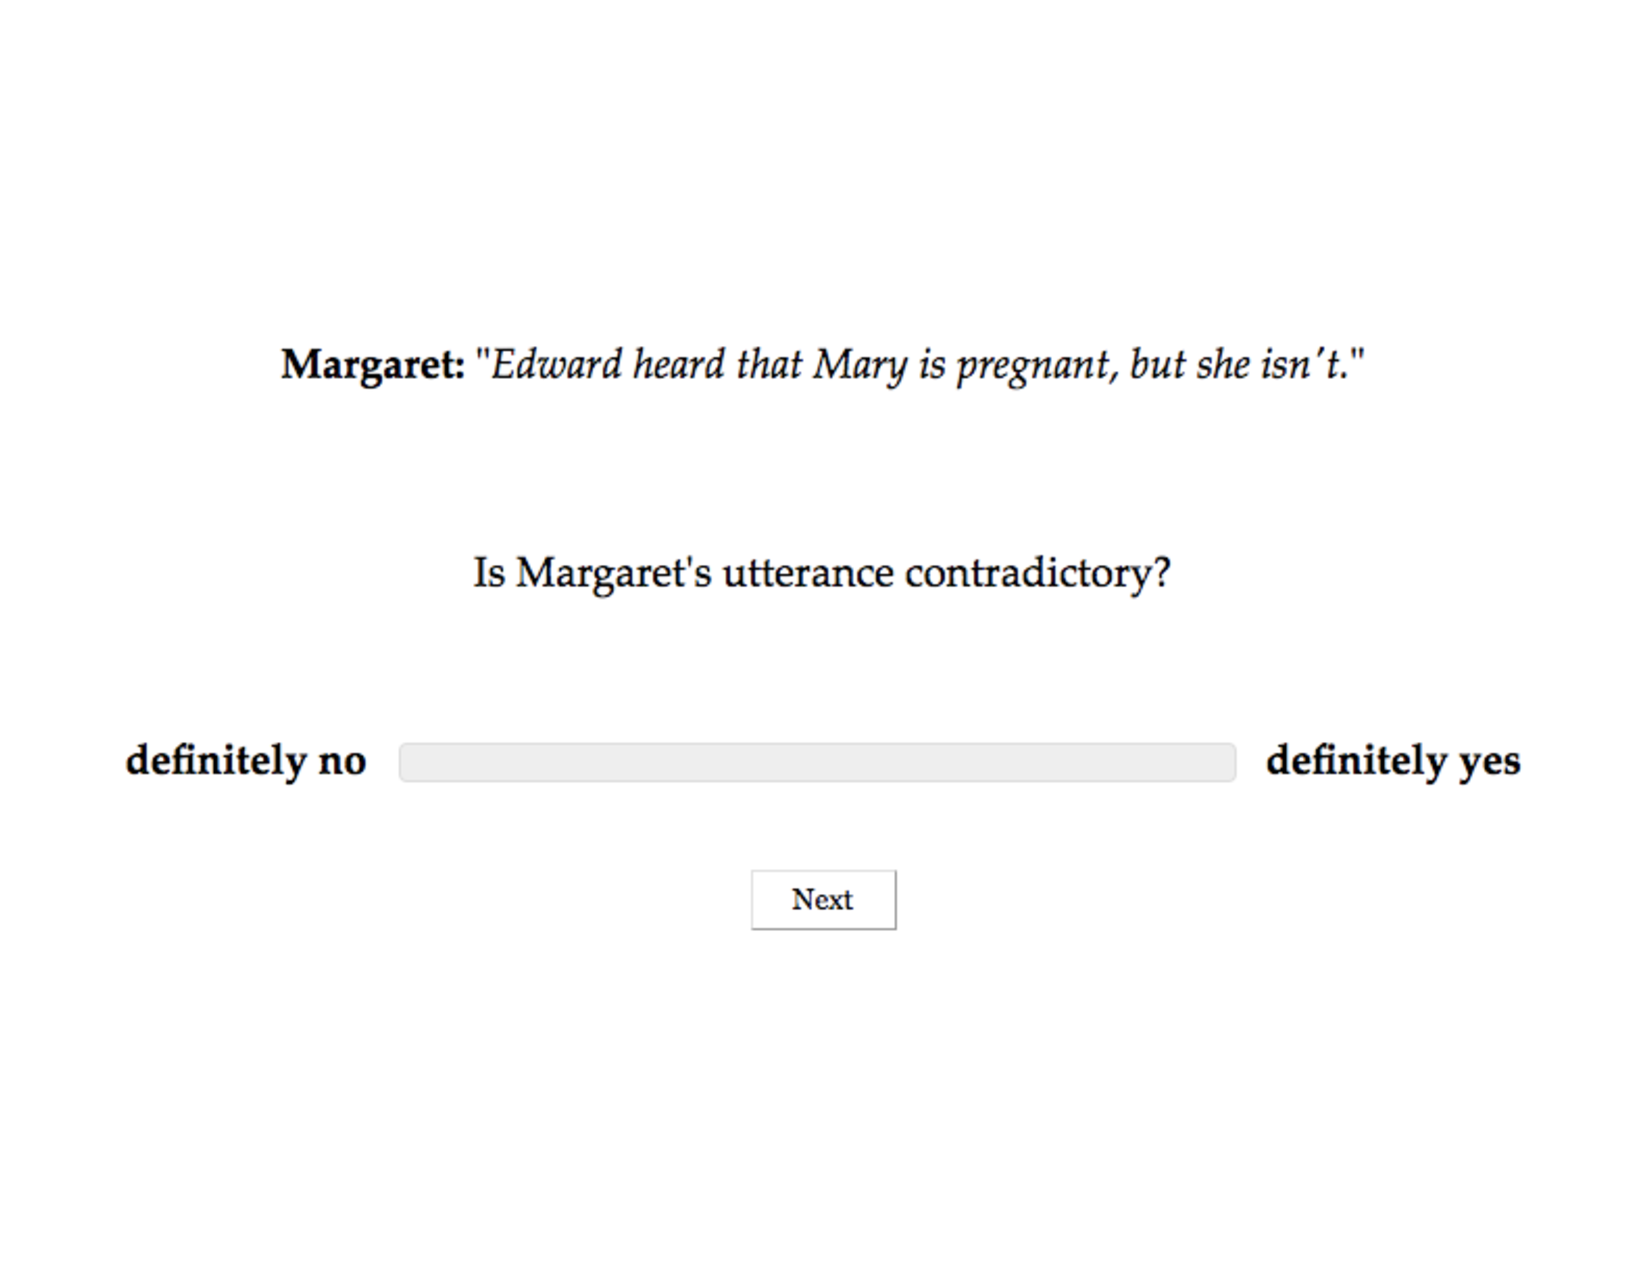
\includegraphics[width=13cm]{figures/contradictory-trial}}
\end{center}
\caption{A sample trial in Experiment 2b}\label{f-trial-exp2}
\end{figure}

To familiarize participants with the task, they first responded to the two familiarization stimuli in (\ref{train}): participants who rated (\ref{train}a) in the lower half of the scale or (\ref{train}b) in the upper half of the scale were given an explanation for why their answer was wrong. Participants could only advance to the 28 stimuli if they gave a plausible rating to the two training stimuli, i.e., a rating in the upper half of the scale for (\ref{train}b) and a rating in the lower half of the scale for (\ref{train}b).

\begin{exe}
\ex\label{train}
\begin{xlist}
\ex Drew is aware that Patty lives in Canada, but she doesn't.

\ex Drew thinks that Patty lives in Canada, but she doesn't.
\end{xlist}
\end{exe}

After responding to the 28 stimuli, participants filled out a short, optional survey about their age, their gender, their native language(s) and, if English is their native language, whether they are a speaker of American English (as opposed to, e.g., Australian or Indian English). To encourage them to respond truthfully, participants were told that they would be paid no matter what answers they gave in the survey.

\paragraph{Data exclusion}

Prior to analysis, the data from 19 participants who did not self-identify as native speakers of American English were excluded. For the remaining 281 participants, we inspected their responses to the 8 control stimuli: as expected, the group mean rating for the non-contradictory control stimuli in (\ref{control-good}) was at floor (.08)\footnote{The mean rating of the non-contradictory control stimulus that was of the same form as the target stimuli, namely (\ref{control-good}a) {\em Zack believes that I'm married, but I'm actually single}, was higher, at .17, than the mean ratings of the remaining three non-contradictory control stimuli (means: .05 or .06). In fact, the mean contradictoriness rating of this control stimulus was identical to that of the target stimuli with {\em think}. The observation that the mean contradictoriness ratings of sentences of the form `NP {\em believe/think} S but not S' was not at floor suggests that it is not as easy for participants to imagine a situation in which such sentences are true as for the other 3 control stimuli. The findings reported on in this section do not change qualitatively if participants are not excluded based on their contradictoriness rating of (\ref{control-good}a). \jt{Does this make sense? If yes, redo the entire analysis by not considering (\ref{control-good}a).}}  and the group mean rating for the contradictory control stimuli in (\ref{control-bad}) was at ceiling (.94). This finding shows that, overall, participants attended to and understood the task; in particular, participants overall gave high contradictoriness ratings to the control stimuli in (\ref{control-bad}) where the first clause entails the negation of the second clause. The mean ratings of 12 participants were more than 3 standard deviations above the group mean for the non-contradictory control stimuli or below the group mean for the contradictory control stimuli. Closer inspection revealed that these participants' responses to the control stimuli were systematically higher or lower, suggesting that these participants did not attend to the task or interpreted the task differently. The data from these 12 participants were also excluded, leaving data from 269 participants (ages 18-72; median: 36; 128 female, 140 male, 1 other) and resulting in new group means of .06 for the control stimuli in (\ref{control-bad}) and .95 for the control stimuli in (\ref{control-good}b). 

\subsubsection{Results}

Each predicate received 269 ratings and each predicate/clause combination received between 3 and 22 ratings (mean: 13.45). The box plot in Figure \ref{f-veridicality-predicate} shows participants' contradictoriness ratings by predicate, collapsing over the 20 complement clauses. The `plain non-factive' predicates {\em pretend, think, suggest} and {\em say} received among the lowest ratings overall, as expected from the assumption that the content of the complement of these predicates is not entailed. We also note that the inference ratings for the `projective non-factive' predicate {\em hear} were quite low, suggesting, as discussed in section \ref{s2}, that participants indeed interpreted the target stimuli with {\em hear} using the evidential sense of {\em hear}, not the sensory sense of {\em hear}. The only predicate whose mean and median contradictoriness ratings are at ceiling is the `veridical non-factive' predicate {\em be right} (mean: .93; median: .98), suggesting that participants took target stimuli with {\em be right} to be highly contradictory. This finding supports an analysis of the content of the complement of {\em be right} as an entailment. For target stimuli with the `projective non-factive' predicate {\em prove} and the `factive' predicate {\em know}, the median contradictoriness ratings are also at ceiling (.95 and .96, respectively), suggesting half of the participants considered target stimuli with these predicates to be highly contradictory. However, the larger box sizes, longer whisker lengths and lower mean contradictoriness ratings for {\em prove} and {\em know} suggest that participants did not consistently assess the target stimuli with these predicates to be contradictory. The same is true for the remaining `factive' and `veridical non-factive' predicates: the mean contradictoriness ratings are .83 for the `factive' predicate {\em know}, .81 for the `factive' predicate {\em see}, .78 for the `factive' predicate {\em discover}, .72 for the `veridical non-factive' predicate {\em demonstrate}, .64 for the `factive' predicate {\em be annoyed} and .63 for the `factive' predicate {\em reveal}.  These findings do not support an analysis of the content of the clausal complement of these predicates as an entailment.

%          verb  Mean  YMin  YMax
%1  acknowledge 0.668 0.627 0.706
%2        admit 0.710 0.670 0.749
%3     announce 0.451 0.404 0.499
%4   be_annoyed 0.636 0.592 0.677
%5     be_right 0.935 0.916 0.951
%6      confess 0.668 0.626 0.708
%7      confirm 0.764 0.726 0.800
%8  demonstrate 0.719 0.681 0.756
%9     discover 0.781 0.745 0.816
%10   establish 0.719 0.679 0.755
%11        hear 0.239 0.205 0.275
%12      inform 0.470 0.423 0.515
%13        know 0.834 0.804 0.865
%14     pretend 0.219 0.183 0.258
%15       prove 0.854 0.828 0.881
%16      reveal 0.629 0.587 0.672
%17         say 0.367 0.323 0.413
%18         see 0.815 0.783 0.845
%19     suggest 0.258 0.221 0.294
%20       think 0.173 0.141 0.206

%  verb        Median
%   <chr>        <dbl>
% 1 acknowledge 0.780 
% 2 admit       0.810 
% 3 announce    0.360 
% 4 be_annoyed  0.720 
% 5 be_right    0.980 
% 6 confess     0.800 
% 7 confirm     0.890 
% 8 demonstrate 0.840 
% 9 discover    0.900 
%10 establish   0.830 
%11 hear        0.0900
%12 inform      0.470 
%13 know        0.960 
%14 pretend     0.0600
%15 prove       0.950 
%16 reveal      0.760 
%17 say         0.200 
%18 see         0.920 
%19 suggest     0.110 
%20 think       0.0300

\begin{figure}[h!]
\centering

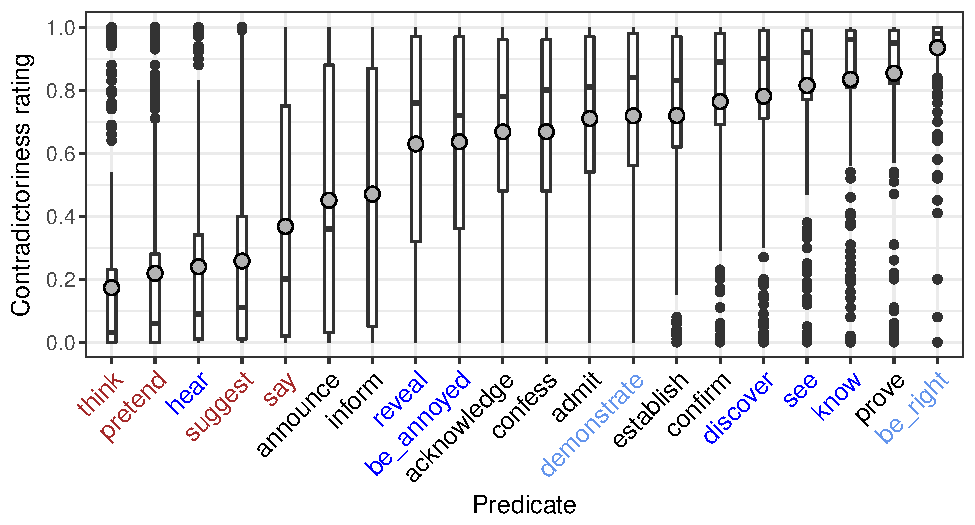
\includegraphics[width=.75\paperwidth]{../results/2-veridicality2/graphs/boxplot-veridicality}

\caption{Box plot of contradictoriness ratings by predicate, collapsing across complement clauses. Grey dots indicate means and notches indicate medians. `Factive' predicates are given in darker blue, `veridical non-factive' ones in lighter blue, `plain non-factive' ones in brown and `projective non-factive' ones in black. {\bf FIX COLOR OF HEAR}}
\label{f-veridicality-predicate}
\end{figure}

To determine which clause-embedding predicates differed from each other in the contradictoriness ratings, we conducted post hoc pairwise comparisons using Tukey's method (allowing for by-participant variability), using the \verb|lsmeans| package \citep{tukey} in R \citep{r}. We included the control stimuli in (\ref{control-bad}) in the analysis to identify predicates for which the contradictoriness ratings are at ceiling (6456 data points total). The $p$-values for each comparison pair are shown in Table  \ref{t-pairwise}. These results suggest no difference in the contradictoriness ratings for the controls in (\ref{control-bad}) and the content of the complement of the `veridical non-factive' predicate {\em be right}. This finding supports an analysis of the content of the complement of {\em be right} as an entailment. {\bf DO WE WANT TO INCLUDE THE CONTROLS? RESULTS CHANGE}


\begin{table}[h!]
\setlength\tabcolsep{3pt}

\centering
\small

\begin{tabular}{l l l l l l l l l l l l l l l l l l l l l}
\toprule

 &   \rot{\color{brown}{\em think}\color{black}} & \rot{\color{brown}{\em pretend}\color{black}} & \rot{\color{blue}{\em hear}\color{black}} &  \rot{\color{brown}{\em suggest}\color{black}} &  \rot{\color{brown}{\em say}\color{black}} & \rot{{\em announce}} & \rot{{\em inform}} & \rot{\color{blue}{\em reveal}\color{black}} & \rot{\color{blue}{\em be annoyed}\color{black}} & \rot{{\em confess}} & \rot{{\em acknowledge}} & \rot{{\em admit}} & \rot{\color{black}{\em establish}\color{black}}  & \rot{\color{airforceblue}{\em demonstrate}}  & \rot{{\em confirm}}  & \rot{\color{blue}{\em discover}\color{black}} & \rot{\color{blue}{\em see}\color{black}}  & \rot{\color{blue}{\em know}\color{black}}  & \rot{{\em prove}} & \\
\midrule
%\color{brown}{\em think}\color{black}		& -- & - & - & - & - & - & - & - & - & - & - & - & - & - & - & - & - & - & - \\
\color{brown}{\em pretend}\color{black}		& n.s. & - & - & - & - & - & - & - & - & - & - & - & - & - & - & - & - & - & - \\
\color{blue}{\em hear}\color{black}			& n.s. & n.s. & - & - & - & - & - & - & - & - & - & - & - & - & - & - & - & - & - \\
\color{brown}{\em suggest}	\color{black}		& * & n.s. & n.s. & - & - & - & - & - & - & - & - & - & - & - & - & - & - & - & - \\
\color{brown}{\em say}\color{black}		& *** & *** & *** & ** & - & - & - & - & - & - & - & - & - & - & - & - & - & - & - \\
\color{black}{\em announce}\color{black}		& *** & *** & *** & *** & * & - & - & - & - & - & - & - & - & - & - & - & - & - & - \\
\color{black}{\em inform}\color{black}		& *** & *** & *** & *** & ** & n.s. & - & - & - & - & - & - & - & - & - & - & - & - & - \\
\color{blue}{\em reveal}\color{black}		& *** & *** & *** & *** & *** & *** & *** & - & - & - & - & - & - & - & - & - & - & - & - \\
\color{blue}{\em be annoyed}\color{black}		& *** & *** & *** & *** & *** & *** & *** & n.s. & - & - & - & - & - & - & - & - & - & - & - \\
\color{black}{\em confess}\color{black}		& *** & *** & *** & *** & *** & *** & *** & n.s. & n.s. & - & - & - & - & - & - & - & - & - & - \\
\color{black}{\em acknowledge}\color{black}	& *** & *** & *** & *** & *** & *** & *** & n.s. & n.s. & n.s. & - & - & - & - & - & - & - & - & - \\
\color{black}{\em admit}\color{black}			& *** & *** & *** & *** & *** & *** & *** & * & . & n.s. & n.s. & - & - & - & - & - & - & - & - \\
\color{black}{\em establish}\color{black}		& *** & *** & *** & *** & *** & *** & *** & ** & * & n.s. & n.s. &  ns & - & - & - & - & - & - & - \\
\color{airforceblue}{\em demonstrate}\color{black}	& *** & *** & *** & *** & *** & *** & *** & ** & * & n.s. & n.s. & n.s. & n.s. & - & - & - & - & - & - \\
\color{black}{\em confirm}\color{black}		& *** & *** & *** & *** & *** & *** & *** & *** & *** & ** & ** & n.s. & n.s. & n.s. & - & - & - & - & - \\
\color{blue}{\em discover}\color{black}		& *** & *** & *** & *** & *** & *** & *** & *** & *** & ** & ** & n.s. & n.s. & n.s. & n.s. & - & - & - & - \\
\color{blue}{\em see}\color{black}			& *** & *** & *** & *** & *** & *** & *** & *** & *** & *** & *** & ** & ** & ** & n.s. & n.s. & - & - & - \\
\color{blue}{\em know}\color{black}			& *** & *** & *** & *** & *** & *** & *** & *** & *** & *** & *** & *** & *** & *** & n.s. & n.s. & n.s. & - & - \\
\color{black}{\em prove}\color{black}			& *** & *** & *** & *** & *** & *** & *** & *** & *** & *** & *** & *** & *** & *** & ** & n.s. & n.s. & n.s. & -  \\
\color{airforceblue}{\em be right}\color{black}		& *** & *** & *** & *** & *** & *** & *** & *** & ***  & ***  & *** & *** & *** & *** & *** & *** & *** & ** & *  \\
\color{black}controls (\ref{control-bad})\color{black}		& *** & *** & *** & *** & *** & *** & *** & *** & ***  & ***  & *** & *** & *** & *** & *** & *** & *** & ** & *  & ?? \\

\bottomrule
\end{tabular}
\caption{P-values associated with pairwise comparison of contradictoriness ratings of clause-embedding predicates and the controls in (\ref{control-bad}) using Tukey's method. `***' indicates significance at .0001, `**' at .01, `*' at .05, `.' marginal significance at .1, and `ns' indicates no significant difference in means. `Factive' predicates are given in darker blue, `veridical non-factive' ones in lighter blue, `plain non-factive' ones in brown and `projective non-factive' ones in black.}\label{t-pairwise}
\end{table}

%\begin{table}[h!]
%\setlength\tabcolsep{3pt}
%
%\centering
%\small
%
%\begin{tabular}{l l l l l l l l l l l l l l l l l l l l }
%\toprule
%
% &   \rot{\color{brown}{\em think}\color{black}} & \rot{\color{brown}{\em pretend}\color{black}} & \rot{\color{blue}{\em hear}\color{black}} &  \rot{\color{brown}{\em suggest}\color{black}} &  \rot{\color{brown}{\em say}\color{black}} & \rot{{\em announce}} & \rot{{\em inform}} & \rot{\color{blue}{\em reveal}\color{black}} & \rot{\color{blue}{\em be annoyed}\color{black}} & \rot{{\em confess}} & \rot{{\em acknowledge}} & \rot{{\em admit}} & \rot{\color{black}{\em establish}\color{black}}  & \rot{\color{airforceblue}{\em demonstrate}}  & \rot{{\em confirm}}  & \rot{\color{blue}{\em discover}\color{black}} & \rot{\color{blue}{\em see}\color{black}}  & \rot{\color{blue}{\em know}\color{black}}  & \rot{{\em prove}}  \\
%\midrule
%%\color{brown}{\em think}\color{black}		& -- & - & - & - & - & - & - & - & - & - & - & - & - & - & - & - & - & - & - \\
%\color{brown}{\em pretend}\color{black}		& n.s. & - & - & - & - & - & - & - & - & - & - & - & - & - & - & - & - & - & - \\
%\color{blue}{\em hear}\color{black}			& n.s. & n.s. & - & - & - & - & - & - & - & - & - & - & - & - & - & - & - & - & - \\
%\color{brown}{\em suggest}	\color{black}		& * & n.s. & n.s. & - & - & - & - & - & - & - & - & - & - & - & - & - & - & - & - \\
%\color{brown}{\em say}\color{black}		& *** & *** & *** & ** & - & - & - & - & - & - & - & - & - & - & - & - & - & - & - \\
%\color{black}{\em announce}\color{black}		& *** & *** & *** & *** & * & - & - & - & - & - & - & - & - & - & - & - & - & - & - \\
%\color{black}{\em inform}\color{black}		& *** & *** & *** & *** & ** & n.s. & - & - & - & - & - & - & - & - & - & - & - & - & - \\
%\color{blue}{\em reveal}\color{black}		& *** & *** & *** & *** & *** & *** & *** & - & - & - & - & - & - & - & - & - & - & - & - \\
%\color{blue}{\em be annoyed}\color{black}		& *** & *** & *** & *** & *** & *** & *** & n.s. & - & - & - & - & - & - & - & - & - & - & - \\
%\color{black}{\em confess}\color{black}		& *** & *** & *** & *** & *** & *** & *** & n.s. & n.s. & - & - & - & - & - & - & - & - & - & - \\
%\color{black}{\em acknowledge}\color{black}	& *** & *** & *** & *** & *** & *** & *** & n.s. & n.s. & n.s. & - & - & - & - & - & - & - & - & - \\
%\color{black}{\em admit}\color{black}			& *** & *** & *** & *** & *** & *** & *** & * & . & n.s. & n.s. & - & - & - & - & - & - & - & - \\
%\color{black}{\em establish}\color{black}		& *** & *** & *** & *** & *** & *** & *** & ** & * & n.s. & n.s. &  ns & - & - & - & - & - & - & - \\
%\color{airforceblue}{\em demonstrate}\color{black}	& *** & *** & *** & *** & *** & *** & *** & ** & * & n.s. & n.s. & n.s. & n.s. & - & - & - & - & - & - \\
%\color{black}{\em confirm}\color{black}		& *** & *** & *** & *** & *** & *** & *** & *** & *** & ** & ** & n.s. & n.s. & n.s. & - & - & - & - & - \\
%\color{blue}{\em discover}\color{black}		& *** & *** & *** & *** & *** & *** & *** & *** & *** & ** & ** & n.s. & n.s. & n.s. & n.s. & - & - & - & - \\
%\color{blue}{\em see}\color{black}			& *** & *** & *** & *** & *** & *** & *** & *** & *** & *** & *** & ** & ** & ** & n.s. & n.s. & - & - & - \\
%\color{blue}{\em know}\color{black}			& *** & *** & *** & *** & *** & *** & *** & *** & *** & *** & *** & *** & *** & *** & n.s. & n.s. & n.s. & - & - \\
%\color{black}{\em prove}\color{black}			& *** & *** & *** & *** & *** & *** & *** & *** & *** & *** & *** & *** & *** & *** & ** & n.s. & n.s. & n.s. & -  \\
%\color{airforceblue}{\em be right}\color{black}		& *** & *** & *** & *** & *** & *** & *** & *** & ***  & ***  & *** & *** & *** & *** & *** & *** & *** & ** & *  \\
%
%\bottomrule
%\end{tabular}
%\caption{P-values associated with pairwise comparison of contradictoriness ratings of predicates using Tukey's method. `***' indicates significance at .0001, `**' at .01, `*' at .05, `.' marginal significance at .1, and `ns' indicates no significant difference in means. `Factive' predicates are given in darker blue, `veridical non-factive' ones in lighter blue, `plain non-factive' ones in brown and `projective non-factive' ones in black.}\label{t-pairwise}
%\end{table}

\newpage

\subsection{Discussion}\label{s33}

\begin{exe}
\exi{(\ref{erq})} Research questions about entailment
\begin{xlist}
\ex Is the content of the complement of `factive' and `veridical non-factive' predicates entailed?

\ex Is the content of the complement of `plain factive' and `projective non-factive' predicates entailed?

\ex Does entailment distinguish `factive' and `veridical non-factive' from `plain non-factive' and `projective non-factive' predicates?
\end{xlist}
\end{exe}

The experiments reported on in the preceding two sections applied two standard diagnostics for entailment to the content of the clausal complement of 20 clause-embedding predicates, with the goal of identifying predicates whose clausal complement is an entailment. Table \ref{t-summary} summarizes the findings of the two experiments under the assumption that the content of the clausal complement of a clause-embedding predicate is an entailment if and only if the strength of the inference to the content is at ceiling (Exp.~2a) and the contradictoriness of utterances of sentences of the form `NP P S but not S' is at ceiling (Exp.~2b). A checkmark `$\checkmark$' indicates that the content of the clausal complement of the clause-embedding predicate is an entailment according to the diagnostic; an `x' indicates that it is not. By the two entailment diagnostics, the `veridical non-factive' predicate {\em be right} is the only predicate for which both experiments provide empirical support for an analysis of the clausal complement as an entailment: Exp.~2a found that the strength of the inference to the content of the clausal complement of {\em be right} is at ceiling and Exp.~2b found that the contradictoriness of sentences of the form `NP {\em is right} S but not S' is at ceiling. 



\begin{table}[h!]
\setlength\tabcolsep{3pt}

\centering
\small

\begin{tabular}{l c c}
\toprule
& \multicolumn{2}{c}{Entailment?} \\ 
& Exp.~2a & Exp.~2b \\ 

\midrule
\color{brown}{\em think}\color{black}		&  x &   x  \\ 
\color{brown}{\em pretend}\color{black}	&    x  &   x  \\ 

\color{brown}{\em suggest}	\color{black}&    x  &   x  \\
\color{brown}{\em say}\color{black}		&    x  &   x  \\ 
\color{black}{\em announce}\color{black}	&    x  &   x  \\ 
\color{black}{\em inform}\color{black}		&    x  &   x  \\ 
\color{black}{\em confess}\color{black}		&   x  &   x  \\ 
\color{blue}{\em hear}\color{black}		&    x  &   x  \\ 
\color{blue}{\em reveal}\color{black}		&    x  &   x  \\ 
\color{airforceblue}{\em demonstrate}\color{black} &	  x  &   x  \\ 


\multicolumn{3}{c}{\makebox[5cm]{\dashrule[black]}} \\[-\jot]

\color{black}{\em acknowledge}\color{black}	& $\checkmark$ & x \\ 
\color{black}{\em admit}\color{black}			& $\checkmark$ & x \\ 
\color{black}{\em confirm}\color{black}		&  $\checkmark$ &  x\\ 
\color{black}{\em prove}\color{black}			&  $\checkmark$ &  x\\ 
\color{black}{\em establish}\color{black}	& $\checkmark$ &  x\\ 

\color{blue}{\em be annoyed}\color{black}		& $\checkmark$ & x \\ 
\color{blue}{\em know}\color{black}			& $\checkmark$  &  x\\ 
\color{blue}{\em discover}\color{black}		&  $\checkmark$ &  x\\ 
\color{blue}{\em see}\color{black}			&  $\checkmark$ &  x\\ 

\multicolumn{3}{c}{\makebox[5cm]{\dashrule[black]}} \\[-\jot]

\color{airforceblue}{\em be right}\color{black}	& $\checkmark$  & $\checkmark$ \\ 
\bottomrule
\end{tabular}
\caption{Findings of Exps.~2a and 2b for the 20 clause-embedding predicates. `Factive' predicates are given in darker blue, `veridical non-factive' ones in lighter blue, `non-factive' ones in brown and `apparently factive' ones in black. `$\checkmark$' indicates that the content of the clausal complement of the clause-embedding predicate is an entailment according to the diagnostic; `x' indicates that it is not.}\label{t-summary}
\end{table}

The findings of the two experiments are mixed for the `factive' predicates {\em see, discover, know} and {\em be annoyed}. On the one hand, Exp.~2a showed that the content of the clausal complement of these predicates was consistently taken to follow from true statements with such predicates. This finding supports an analysis of the content of the clausal complement as an entailment. On the other hand, Exp.~2b showed that the contradictoriness of sentences of the form `NP P S but not S' with these predicates was not at ceiling. This finding does not support an analysis of the clausal complement as an entailment. Crucially, these findings are identical to those for the `apparently entailing' predicates {\em prove, confirm, admit, establish} and {\em acknowledge}. In short, the experiment findings do not support a non-arbitrary division between the  `factive' predicates {\em see, discover, know} and {\em be annoyed}, on the one hand, and the `apparently factive' predicates {\em prove, confirm, establish, admit} and {\em acknowledge}, on the other.

Finally, for the `factive' predicates {\em reveal} and {\em hear}, and for the `veridical non-factive' predicate {\em demonstrate}, neither of the two experiments found support for an analysis as a predicate whose clausal complement is entailed. Exp.~2a showed that the content of the clausal complement follows less strongly from true statements with these predicates than from true statements with other `factive' and `veridical non-factive' predicates, and, for {\em hear} and {\em demonstrate}, even less strongly than for some `apparently factive' predicates. Exp.~2b showed that  contradictoriness ratings of sentences of the form `NP P S but not S' with these predicates are lower than many `factive', `veridical non-factive' and `apparently factive' predicates; all of them, in fact, for {\em hear}. Thus, by the findings of Exps.~2a and 2b, an analysis of the content of the clausal complement of {\em reveal, hear} and {\em demonstrate} as an entailment is no more supported than for the `non-factive' predicates, for which the two experiments also didn't find support for an analysis of the clausal complement as an entailment. 

In sum, the findings of the two experiments, which applied standard diagnostics for entailment to 20 clause-embedding predicates, did not finding support that the `factive' and `veridical non-factive' predicates under investigation are a natural class of predicates whose clausal complement is an entailment. 

One possible concern with the two diagnostics is that the findings of the two experiments diverge for a number of predicates: specifically, responses were at ceiling for the content of the clausal complement of the `factive' predicates {\em see, discover, know} and {\em be annoyed} and the `apparently factive' predicates {\em  establish, prove, confirm, admit} and {\em acknowledge} in Exp.~2a but not in Exp.~2b. We believe that this difference is due to a difference in the demand that the two diagnostics placed on the participants. In Exp.~2a, to give a response that was not at ceiling, participants had to identify a situation in which the true sentence (e.g., {\em Mark announced that Sophia got a tattoo}) is true and in which the content of the clausal complement is false. This is a challenging task that required creativity and linguistic acuity of the participants. In Exp.~2b, on the other hand, participants were able to give a contradictoriness response that was not at ceiling as soon as they judged the speaker's utterance (e.g., Tom: {\em Mark announced that Sophia got a tattoo, but she didn't}) to not be entirely odd, i.e., as not being entirely contradictory. This task is considerably less demanding than that of Exp.~2a and, thereby, may have led to more not-at-ceiling responses in Exp.~2b than in Exp.~2a.

Despite this difference between Exps.~2a and 2b, the numerical findings of the two experiments are remarkably parallel: on both diagnostics, target stimuli with {\em pretend, think, hear} and {\em suggest} received the lowest ratings, those with the communicative act predicates {\em say, announce} and {\em inform} received the next-to-lowest ratings and those with {\em prove} and {\em be right} received the highest ratings.\footnote{\jt{JD suggests: maybe also include scatterplot of ratings for exp2a and exp2b to look at correlation as a way of assessing reliability of measures?}
} This observation suggests that the two diagnostics measured the same underlying concept, even if the diagnostic of Exp.~2b made it easier for participants to give not-at-ceiling responses.  


%\begin{figure}[h!]
%\centering
%
%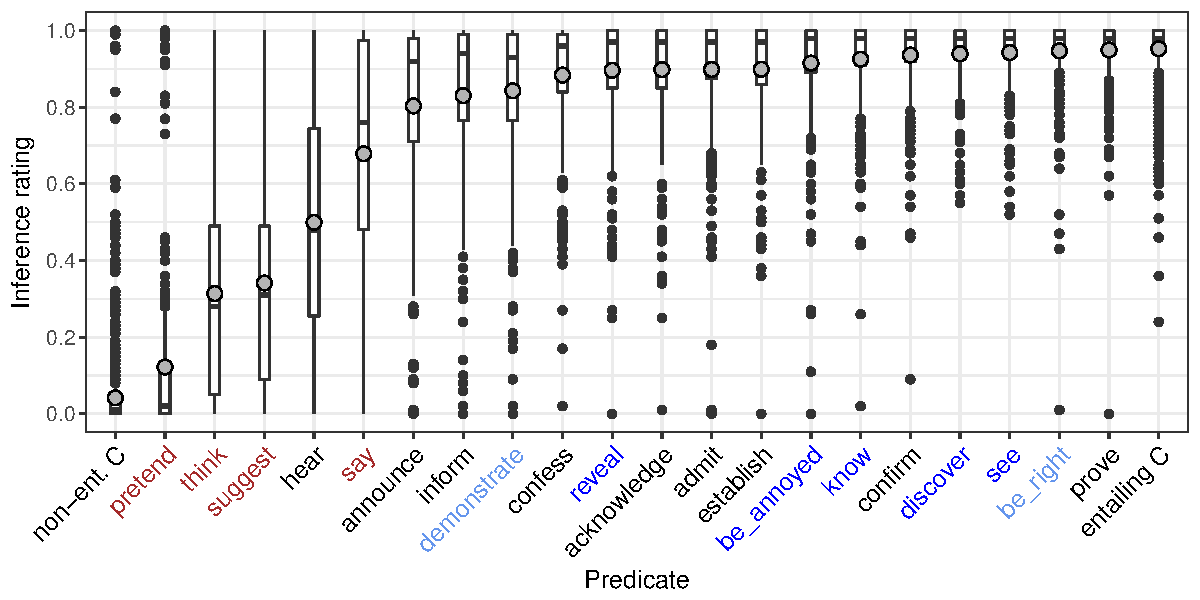
\includegraphics[width=.4\paperwidth]{../results/4-veridicality3/graphs/boxplot-inference}
%
%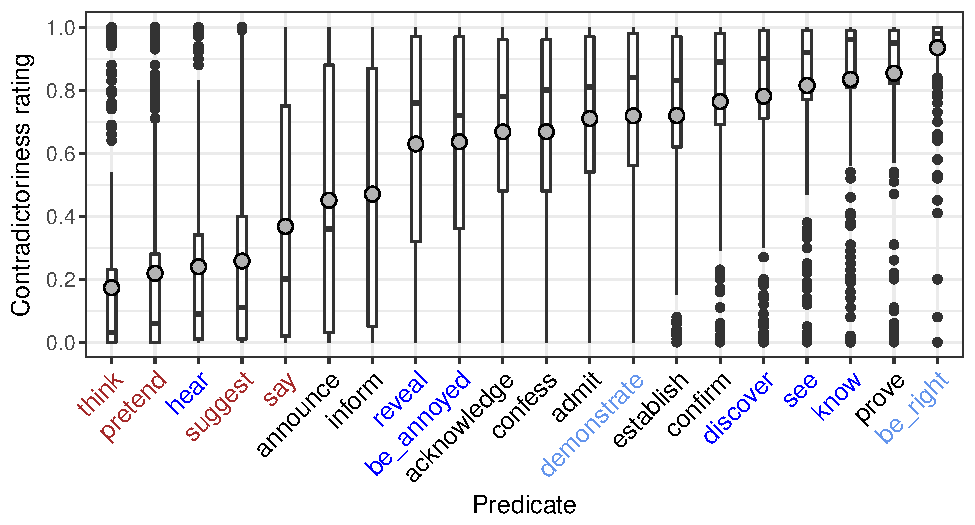
\includegraphics[width=.4\paperwidth]{../results/2-veridicality2/graphs/boxplot-veridicality}
%
%\caption{Box plot of contradictoriness ratings by predicate, collapsing over complement clauses. Grey dots indicate means and notches indicate medians. `Factive' predicates are given in darker blue, `veridical non-factive' ones in lighter blue, `non-factive' ones in brown and `apparently factive' ones in black.}
%\label{f-veridicality-predicate}
%\end{figure}

Another potential concern with the validity of the two diagnostics for entailment in Exps.~2 is that they were implemented with gradient rather than binary response tasks. Is it possible that the `factive' and `veridical non-factive' predicates did not emerge as a natural class from the two experiments because participants were asked to give their response on a sliding scale rather than forced to make a binary choice? To investigate this possibility, we recoded participants' responses in the two experiments.


We want to be very clear here that our experiments have {\bf not} shown that clause-embedding predicates cannot be classified into ones whose clausal complement is an entailment and ones whose clausal complement is not an entailment. Rather, our experiments have merely shown that two standard diagnostics for entailment do not provide empirical support for such a lexical classification of clause-embedding predicates. 

It is possible, of course, that there is a diagnostic for entailment that may be better suited to identifying a natural class of clause-embedding predicates whose clausal complements are entailments. 


How reliable and valid are the two diagnostics for entailment of Exps.~2a and 2b? 

 The burden of proof, however, now lies with researchers who want to maintain such a lexical division of clause-embedding predicates. 

\jt{I think the first critique that we are going to get is something like this: ``of course the results are not at ceiling/gradient for Exp. 2b, given that you used a gradient response task. things would look different if you only offered a binary choice `contradictory' vs `not contradictory'. I think we should stave this off by running a smaller version of Exp 2b with such a binary response task. If you agree, how to we scale it down? E.g., only run the 20 predicates with 10 clauses but only 100 participants. Or should we run another full experiment with 300 participants?}

\section{Discussion}\label{s4}

the results do not support a non-arbitrary division of predicates into those for which the content of the clausal complement projects and those for which it doesn't.  Rather, the findings motivate an utterance-level analysis of projectivity: the speaker of any given utterance is taken to be committed to the content of the clausal complement to a particular degree and the clause-embedding predicate is one factor that influences how projective the content is (see also \citealt{tbd-variability}). Other factors include information structure (e.g., \citealt{cummins-rohde2015,tonhauser-salt26,djaerv-bacovcin-salt27}), at-issueness (\citealt{tbd-variability}) and common ground information (\citealt{gazdar79a,tonhauser-etal-eval}).


let's just get rid of the requirement of entailment: heim's analysis fails, but for abrusan and simons et al we could then say that when the complement is contextually entailed (e.g., because trustworthy speaker), it participates in projection process

\begin{verbatim}
- are presuppositions entailments?

	- there is disagreement in the literature about whether presuppositions are entailments or not. to some extent, this is about a difference in whether "entailment" is taken to be an empirical generalization, supported by judgments, or also a theoretical concept; entailment is something we can empirically asses; there's no reason to say that "know" doesn't entail content of clausal complement; we need to distinguish between empirical facts (follows from) and how we account for them (e.g., whether complement is entailed and presupposed, or only presupposed)
	
	- presuppositions are entailments: Stalnaker 1974, Atlas 1975a, (factive sentences), Atlas \& Levinson 1981, Abrusan 2011
	
		- Atlas & Levinson 1981:2 "Whenever "presuppositions" occur...the propositions should be considered an entailment of the affirmative sentence and part of or entailed by a generalized conversational implicatum of saying the negative sentence."
		
		- Gazdar 1979:120: considers factive sentences to entail content of complement
		
	- presuppositions are not entailments	
	
		- Strawson 1950:330: A speaker uttering "The king of France is wise" implies that the speaker believes that there is a king of France. It doesn't entail (logically imply) that there is a king of France, because, when somebody responds with "There is no king of France", this should not mean that they are contradicting "The king of France is wise" (speaker utters "p & q"; responder saying "not-p" would mean "not (p&q)" if p was an entailment, on par with q)
		
	- Sudo 2012: presupposition is entailment (continue, stop) or not (also)
	
	- Zehr & Schwarz  2016 (NELS): if presupposition of "stop" is entailed, it should more regularly be part of scope of "exactly 1" than observed
			Exactly one student stopped smoking
			entailed and ps: Exactly one (student) (smoked in the past and doesn't smoke now) 
			presupposed only: Some students smoked in the past and exactly one (student) (doesn't smoke now)
			local accommodation: Exactly one student ?
			
	- really need to highlight that lots of people consider presuppositions as entailed, with entailed content being "merely entailed"
	
	- conversationalist analyses of soft presuppositions assume that presuppositions are entailments that somehow get backgrounded and project 

		- entailment depends on aspect (easier if gradable inference) Falk
		
		- check out factive examples with non-projecting interpretations
		
http://www.chicagotribune.com/news/opinion/commentary/ct-trump-john-bolton-war-20180323-story.html

\end{verbatim}

Presuppositions have traditionally been characterized as content that is backgrounded and taken for granted (e.g., \citealt{stalnaker74,ccmg90}). Under formal analyses of presuppositions, including contents of complements of `factive' predicates, two empirical properties of presuppositions are taken to follow from this characterization: first, presupposed content is entailed content, i.e., it necessarily follows from true statements of positive matrix sentences; second, presupposed content is projective content, i.e., the speaker is typically taken to be committed to the content even when the expression that contributes the content is embedded under an entailment-canceling operator. Importantly, presupposed content is assumed to be entailed regardless of how projectivity is derived, for instance, regardless of whether projectivity arises from a requirement that presupposed content is entailed by or satisfied in the common ground (e.g., \citealt{heim83,vds92}),  is derived  from lexically-specified alternatives (e.g., \citealt{abusch10,romoli2015}), arises from a default main point mechanism (e.g., \citealt{abrusan2011,abrusan2016}) or from the question addressed by the utterance (e.g., \citealt{best-question}). 

This paper explored the presumed veridicality and projectivity of presupposed content on the basis of sentences with clause-embedding predicates: with `factive' predicates, the content of the clausal complement is analyzed as a presupposition, i.e., is taken to be both entailed and projective, and that of `non-factive' predicates is not analyzed as a presupposition. In Exps.~1 and 2, we explored the projectivity and veridicality of the content of the clausal complement of 20 clause-embedding predicates: projectivity was explored using the `certain that' diagnostic and veridicality was explored using two standard diagnostics for entailment, the inference diagnostic and the contradictoriness diagnostic. The findings of Exp.~1 showed that the content of the clausal complement of many `non-factive' predicates is projective, in some cases even more projective than that of `factive' predicates. The findings of Exps.~2  provided unanimous support for an analysis as an entailment only for the content of the clausal complement of {\em be right}. For the other `factive' and `veridical' predicates, there was either only support from the inference diagnostic (e.g., {\em know, be annoyed}) or no support at all ({\em reveal, demonstrate}) for an analysis of the content of the complement as entailed. Crucially, several `apparently factive' predicates patterned like the `factive' and `veridical' predicates. Thus, Exps.~2 did not provide support for a natural class of clause-embedding predicates for which the content of the complement can be analyzed as entailed and, consequently, no natural class of `factive' predicates emerged from Exps.~1 and 2. In short, the experiments did not find empirical support for the presumed distinction between `factive' and `non-factive' predicates.

Where do we go from here? A first possibility, already mentioned at the end of section \ref{s3}, is that there is a better diagnostic for entailment on the basis of which clause-embedding predicates for which the content of the clausal complement is an entailment can be distinguished from ones for which it is not. 


{\bf see and hear indistinguishable in projectivity but only one comes out as veridical ever}



\begin{itemize}

\item What an analysis of the content of the clausal complement of `factive' predicates as a presupposition is supposed to capture is that speaker is taken to be committed to this content, whether complement clause is embedded or not. 

\item The problem is that presuppositions are defined using a binary notion of speaker commitment: either speaker is committed to truth (entailed, projects) or not necessarily committed to truth (not entailed, doesn't project).

\item So what are ways forward? 

1. Better diagnostics for entailment? Seems unlikely because our findings are consistent with previous research on veridicality. \citealt{demarneffe-etal2012}, WHITE

Our experiment findings are entirely consistent with prior research on veridicality. As discussed in \citealt{demarneffe-etal2012}, veridicality judgments are often influenced by context. 

\begin{exe}
\ex A hypothetical sentence in the New York Times: \\ United Widget said that its chairman resigned. \hfill (\citealt[302]{demarneffe-etal2012})
\end{exe}

p.302: Lexical theories of this sort provide a basis for characterizing readers? veridicality judgments, but they do not tell the whole story, because they neglect the pragmatic enrichment that is pervasive in human communication. In the lexical view, say can only be classified as non-veridical (both true and false things can be said), and yet, if a New York Times article contained the sentence United Widget said that its chairman resigned, readers would reliably infer that United Widget?s chairman resigned?the sentence is, in this context, veridical (at least to some degree) with respect to the event described by the embedded clause, with United Widget said functioning to mark the source of evidence (Simons 2007). Cognitive authority, as termed in information science (Rieh 2010), plays a crucial role in how people judge the veridicality of events. Here, the provenance of the document (the New York Times) and the source (United Widget) combine to reliably lead a reader to infer that the author intended to convey that the event really happened. Conversely, allege is lexically non-veridical, and yet this only begins to address the complex interplay of world knowledge and lexical meaning that will shape people?s inferences about the sentence FBI agents alleged in court documents today that Zazi had ad- mitted receiving weapons and explosives training from al Qaeda operatives in Pakistan last year.

p.302, footnote 2: Our use of the term ?veridicality? most closely matches that of Giannakidou (1999), where it is defined so as to be (i) relativized to particular agents or perspectives, (ii) gradable, and (iii) general enough to cover not only facts but also the commitments that arise from using certain referential expressions and aspectual morphology. The more familiar term ?factuality? seems at odds with all three of these criteria, so we avoid it.



2. Give up on the idea that presuppositions are entailments. Problematic for all kinds of analyses: lexicalist, best question, conversational implicature

3. Don't assume presuppositions, but projectivity is what should be explained. Connect explanations to lexical meanings of clause-embedding predicates. E.g., A\&H explanation for verbs of saying. Factors that matter: at-issueness, authority, prior probability. Need to investigate how much each of these properties matter.

\newpage


If, for instance, a projection analysis assumes that the content of the clausal complement to be entailed, then the analysis should only apply to  clausal complements that are, in fact, entailments. It is for this reason that \citet{schlenker10} only takes those utterances of {\em announce} to trigger a presupposition in which the content of the clausal complement is locally entailed.\footnote{\citepos{schlenker10} notion of entailment seems to be context-sensitive one, i.e., not the classical context-insensitive notion whereby a sentence $\phi$ entails a sentence $\psi$ if and only if all situations in which $\phi$ is true are situations in which $\psi$ is true. For instance, he assumes that ``in some contexts, [{\em announce}, JT\&JD] does not entail the truth of its complement; in other contexts, it entails and presupposes the truth of its complement" (p.139).} 

More drastically, \citet{anand-hacquard2014} deny that the projectivity of the content of the clausal complement of {\em announce} and {\em inform} falls into the purview of analyses of presuppositions: for them,  `non-factive' predicates merely give rise to an ``illusion of factivity'' (p.75) and an ``illusion of projection'' (p.76). They argue instead that speaker commitment to the content of the clausal complement of predicates like {\em acknowledge, admit} and {\em confirm} arises from these predicates reporting ``discourse moves which lead to the acceptance of the complement $p$ into the common ground of the reported discourse'' (p.74) and then ``[t]his acceptance of p can easily bleed into the actual common ground'' (p.75). Thus, once the content of the complement of a clause-embedding predicate is determined to not be an entailment, i.e., the predicate is `non-factive', the projectivity of the content of the clausal complement must be derived differently than for `factive' predicates.

It is uncontroversial that projectivity may derive from different sources for different kinds of content: see, for instance, \citealt{potts05} on conventional implicatures, \citealt{beaver-clark08} on the prejacent of {\em only} or \citealt{abrusan2013} on the prejacent of manner adverb utterances.  For the clause-embedding predicates, too, it is possible that the projectivity of the content of the clausal complement should be derived from different sources: for instance, along the lines of \citepos{anand-hacquard2014} proposal for `non-factive' reporting predicates and along the lines of \citealt{abusch10,abrusan2011} and \citealt{romoli2015} for `factive' predicates whose clausal complement is less highly projective. It is critical, therefore, to understand which clausal complements form a natural class. In this paper, we examine whether `factive' predicates form a natural class and, in particular, whether the veridicality and projectivity of the content of the clausal complement of `factive' predicates empirical motivates considering such predicates to form a natural class. We already saw above that projectivity is not a property that distinguishes `factive' from `non-factive' predicates. 

\end{itemize}

\section{Conclusions}\label{s5}

\appendix

\setcounter{table}{0}
\renewcommand{\thetable}{A\arabic{table}}

\setcounter{figure}{0}
\renewcommand{\thefigure}{A\arabic{figure}}

\section{Citations}

That both properties are ascribed to presuppositions, including the content of the complement of `factive' predicates, can be seen from the following quotes:

\begin{itemize}[topsep=0pt,itemsep=-3pt,leftmargin=12pt]

\item \citealt[66f.]{beaver01}: \citet[119-123]{gazdar79a} ``describes the inferences associated with factive verbs, definite descriptions, aspectual verbs, and clefts as being indefeasible in simple affirmative sentences'', i.e., ``entailments''.

\item \citealt[355]{ccmg90}: ``A sentence can both entail and presuppose another sentence [...]. Thus, [{\em Joan realizes that syntax deals with sentence structure}] both entails and presupposes [{\em Syntax deals with sentence struture}]."

\item \citealt[345]{vds92}: ``Note that [global accommodation, i.e., projection, JT\&JD] is what we would expect given the intuitive notion of presupposition as information taken for granted and note also that this explains the intuition that presuppositions [...] are entailed by their matrix sentence.''

\item \citealt[3]{abbott06}: ``we will need to be careful to distinguish entailments that are presupposed from what I will call ``ordinary, simple entailments'', which are not also presuppositions.''

\item \citealt[139]{schlenker10}: ``we obtain the pattern of inference which is characteristic of presuppositions: an entailment of the positive sentence is preserved under negation and in questions''


\item \citealt[77]{anand-hacquard2014}: ``we will adopt the pragmatic view of presupposition triggering, according to which presuppositions are lexical entailments that are backgrounded based on pragmatic principles"

\item {\bf \citealt[fn.7]{spector-egre2015}: Assuming that any presupposition of a sentence is also an entailment of this sentence, it follows that a predicate that is factive with respect to its declarative complement is always also veridical with respect to its declarative complement.}

\end{itemize}

\section{20 complement clauses}\label{a-clauses}

The 20  clauses that realized the complement clauses of the 20 clause-embedding predicates in Experiments 1 and 2 are as follows:

\begin{enumerate}[leftmargin=3ex,itemsep=-2pt]

\begin{multicols}{2}

\item Mary is pregnant.
\item Josie went on vacation to France.
\item Emma studied on Saturday morning.
\item Olivia sleeps until noon.
\item Sophia got a tattoo.
\item Mia drank 2 cocktails last night.
\item Isabella ate a steak on Sunday.
\item  Emily bought a car yesterday.
\item  Grace visited her sister.
\item Zoe calculated the tip.

\columnbreak

\item  Danny ate the last cupcake.
\item  Frank got a cat.
\item  Jackson ran 10 miles.
\item  Jayden rented a car.
\item  Tony had a drink last night.
\item  Josh learned to ride a bike yesterday.
\item  Owen shoveled snow last winter.
\item  Julian dances salsa.
\item  Jon walks to work.
\item  Charley speaks Spanish.

\end{multicols}

\end{enumerate}


\bibliographystyle{/Users/tonhauser.1/Library/Latex/cslipubs-natbib}
\bibliography{/Users/tonhauser.1/Documents/bibliography}

\end{document}

